\documentclass{beamer}

\mode<presentation>
{
  \usetheme{Berkeley}
  \setbeamercovered{transparent}
}

\usepackage[absolute,overlay]{textpos}
\usepackage{graphicx}
\usepackage{color}
\usepackage{epsfig}
\usepackage[english]{babel}
\usepackage{listings}
\usepackage{graphics}
\usepackage{subfigure}

\setlength{\TPHorizModule}{1cm}
\setlength{\TPVertModule}{\TPHorizModule}
\textblockorigin{1cm}{1cm} % start everything near the top-left corner
\setlength{\parindent}{0pt}

\title{Data Dissemination: from Academia to Industry}

\author{\textbf{Jo{\~a}o Leit{\~a}o}\\NOVA-LINCS \& NOVA University of Lisbon
\\\textbf{Jordan West}\\BASHO Inc.
}
\date{RICON\\Las Vegas\\October 2014}

\begin{document}
%\definecolor{links}{rgb}{0.2116,0.0104,0.7716}
%\definecolor{highlight}{rgb}{1,1,0.1}


\frame{

\titlepage

}

\section{Motivation}

\frame
{
	\frametitle{Outline}
{
\tiny
	\tableofcontents[hideallsubsections]
}
}

\frame
{
	\frametitle{Outline}
{
\tiny
	\tableofcontents[currentsection,hideallsubsections]
}
}

\frame{

\frametitle{Motivation}
\framesubtitle{Data Dissemination}

\begin{block}{Classical Distributed Systems Challenge}
How to disseminate information across a large number of participants?
\end{block}

\pause

\begin{itemize}
\item Some intuitive requirements:
\begin{itemize}
	\item Reliable.
	\item Efficient.
	\item Scalable.
\end{itemize}
\end{itemize}

}

\frame{

\frametitle{Motivation}
\framesubtitle{Data Dissemination}

\begin{block}{Applications}
\begin{itemize}
	\item Notification systems.
	\item Streaming multimedia content.
	\item \emph{Cluster Management}
\end{itemize}
\end{block}

\pause

\begin{block}{In practice...}
When I started to think about this problem, I was mostly focused on peer-to-peer systems.
\end{block}}

\section{The Academic View: Data Dissemination}

\frame
{
	\frametitle{Outline}
{
\tiny
	\tableofcontents[currentsection,hideallsubsections]
}
}

\subsection{Design Alternatives: One to All}

\frame{
\frametitle{The Academic View: Data Dissemination}
\framesubtitle{Design Alternatives: One to All}

	\begin{block}{Lets start simple...}
		If you have information to disseminate, send it to everyone!
	\end{block}
	
	\pause
	
	~\\
	
	\begin{center}
	\huge{One to All}
	\end{center}

}

\frame{
\frametitle{The Academic View: Data Dissemination}
\framesubtitle{Design Alternatives: One to All}

\begin{figure}[h]
  \begin{center}
  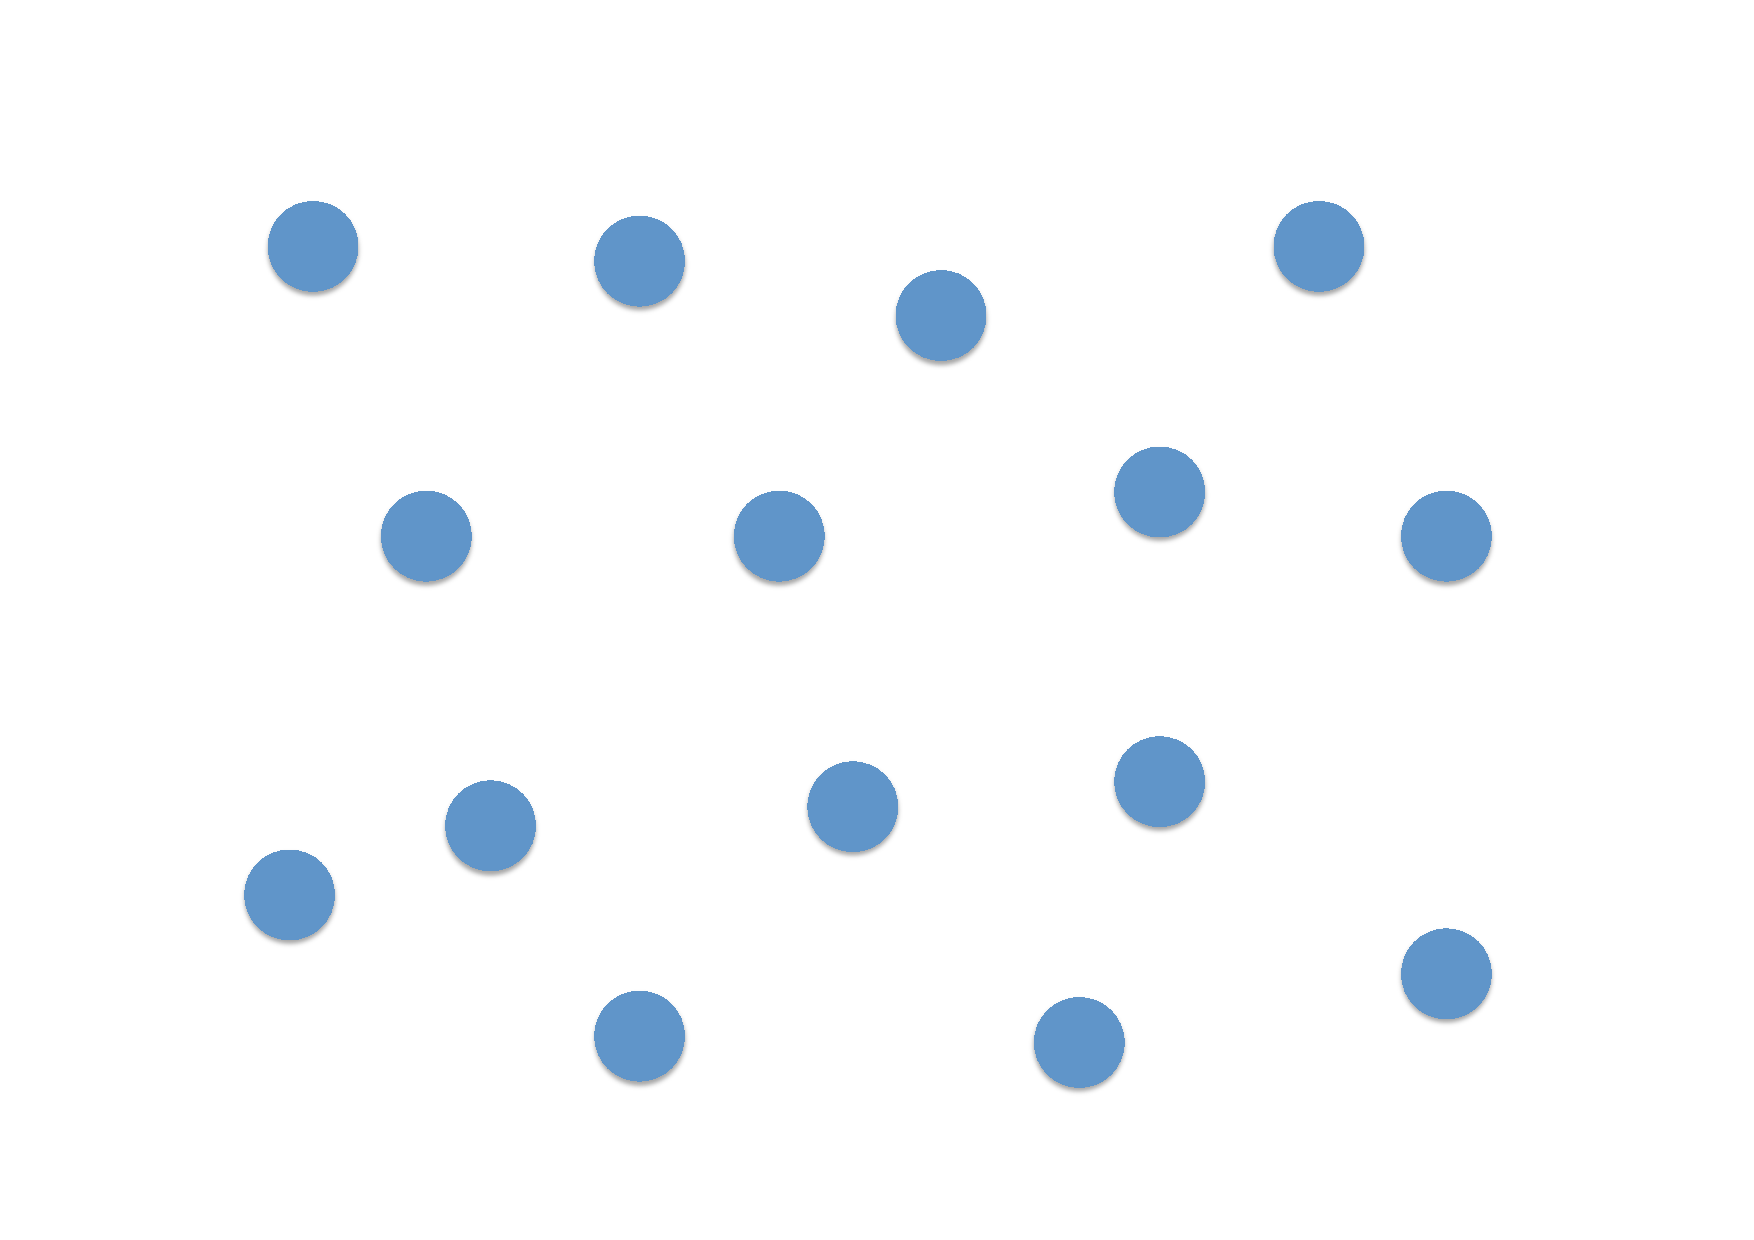
\includegraphics[width=1\textwidth]{pics/one2all1}
  \end{center}
\end{figure}

}

\frame{
\frametitle{The Academic View: Data Dissemination}
\framesubtitle{Design Alternatives: One to All}

\begin{figure}[h]
  \begin{center}
  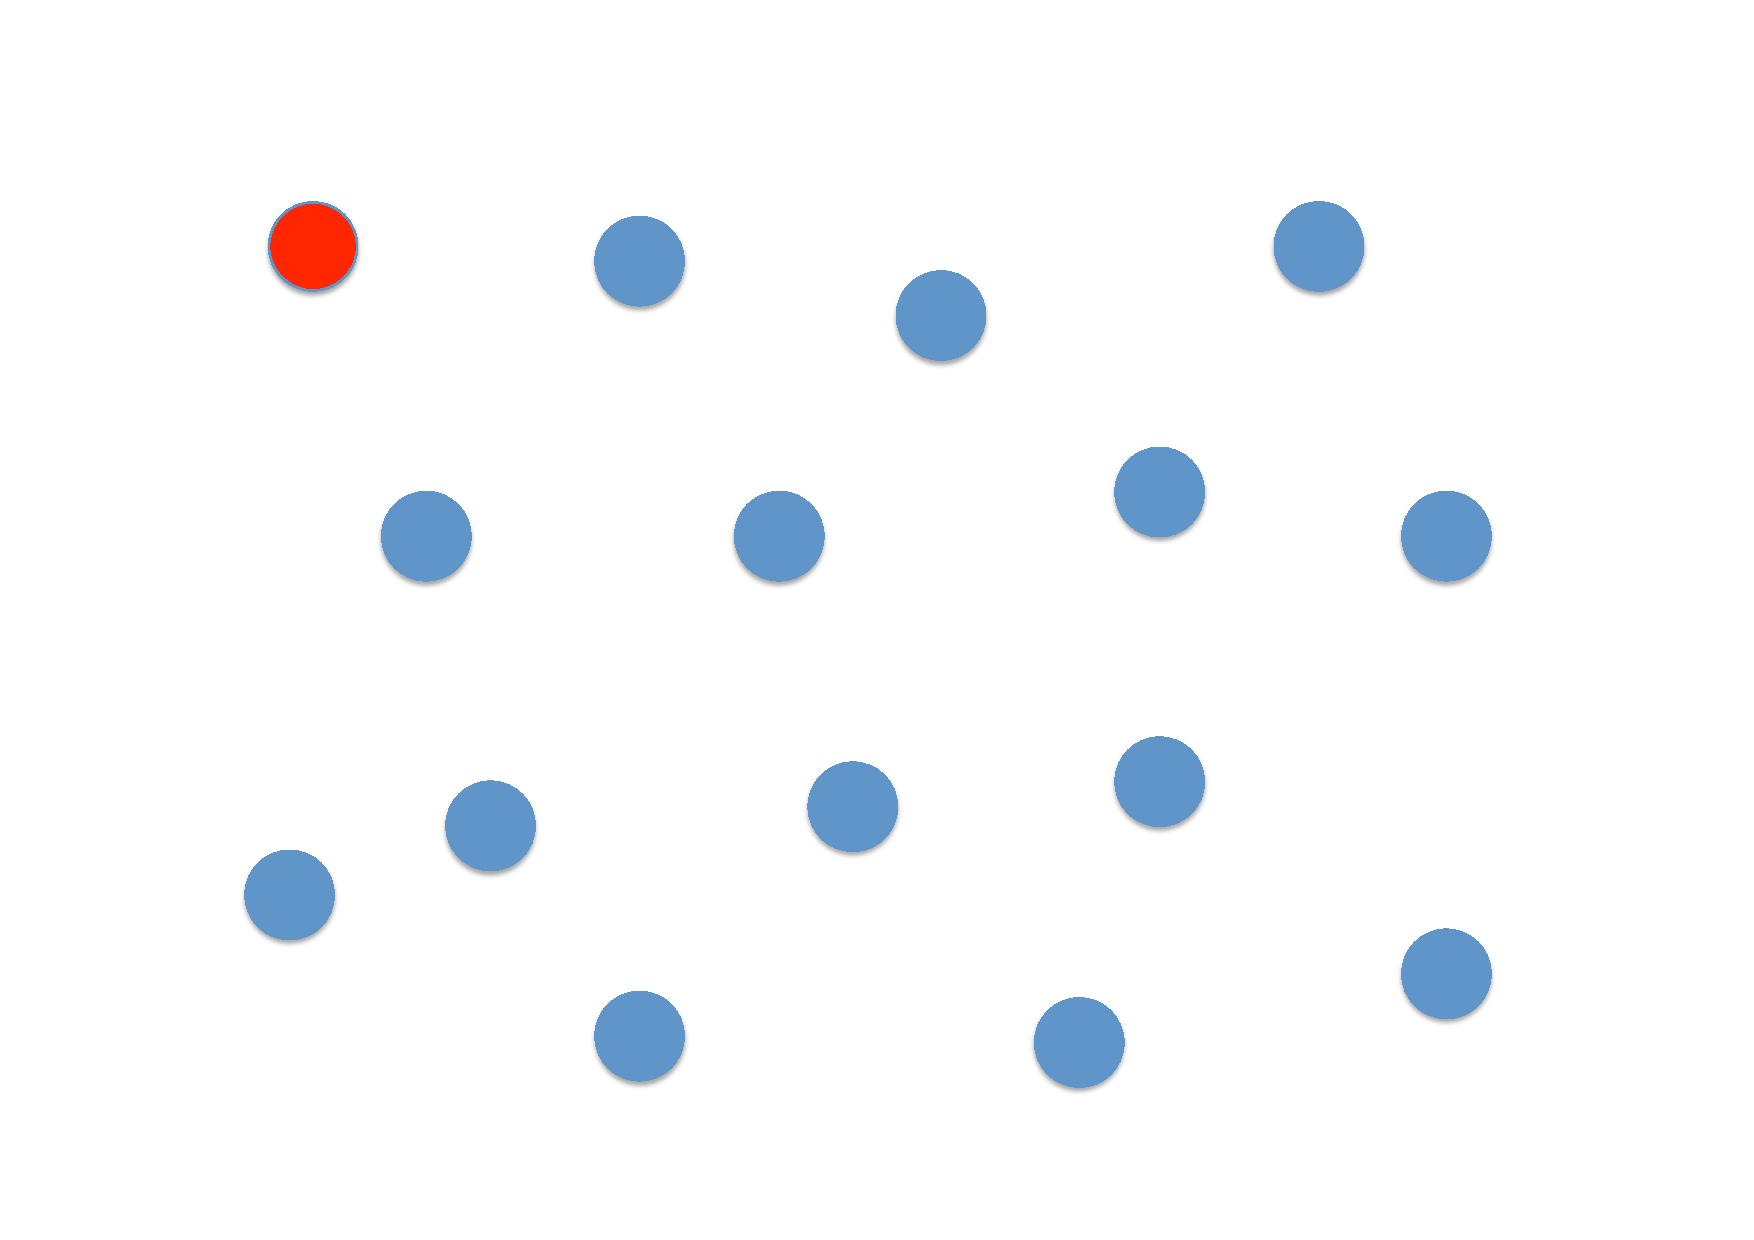
\includegraphics[width=1\textwidth]{pics/one2all2}
  \end{center}
\end{figure}

}

\frame{
\frametitle{The Academic View: Data Dissemination}
\framesubtitle{Design Alternatives: One to All}

\begin{figure}[h]
  \begin{center}
  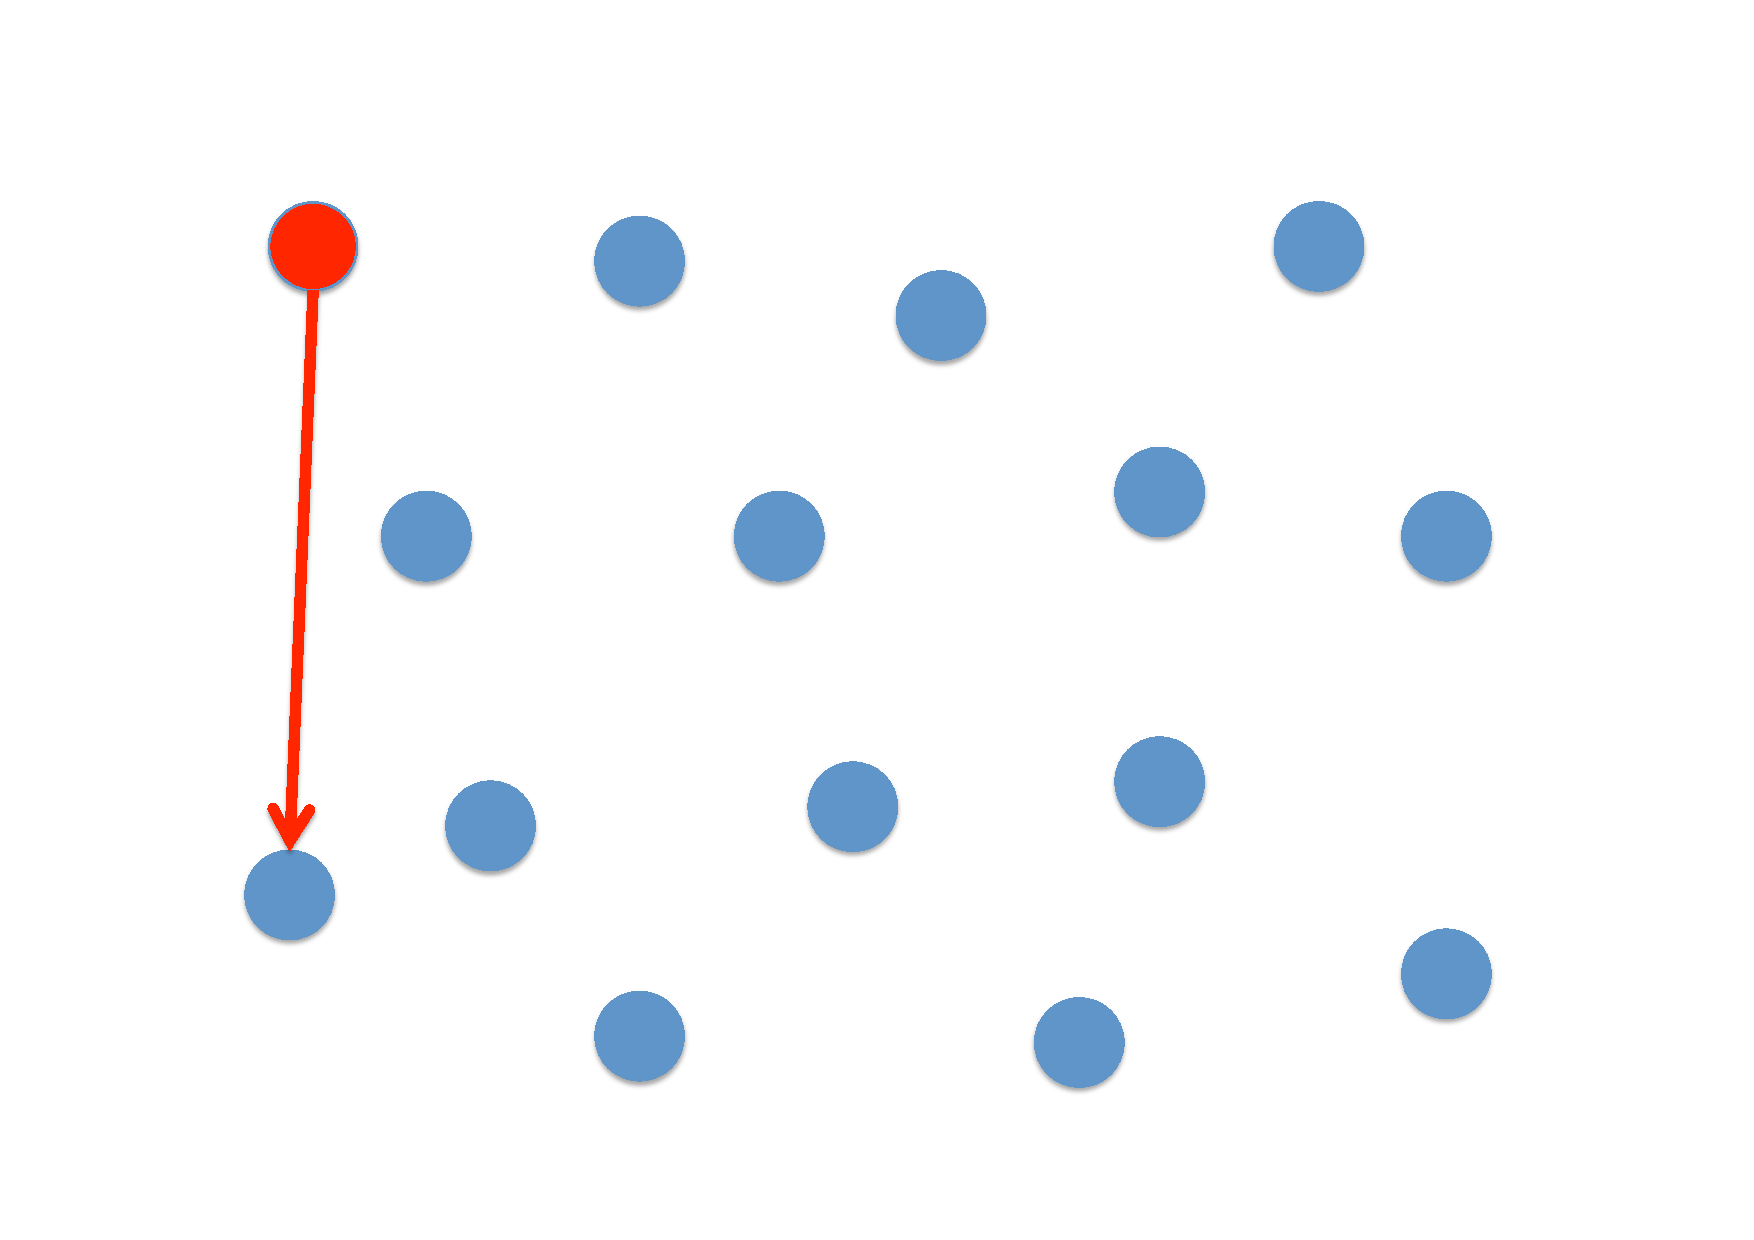
\includegraphics[width=1\textwidth]{pics/one2all3}
  \end{center}
\end{figure}

}

\frame{
\frametitle{The Academic View: Data Dissemination}
\framesubtitle{Design Alternatives: One to All}

\begin{figure}[h]
  \begin{center}
  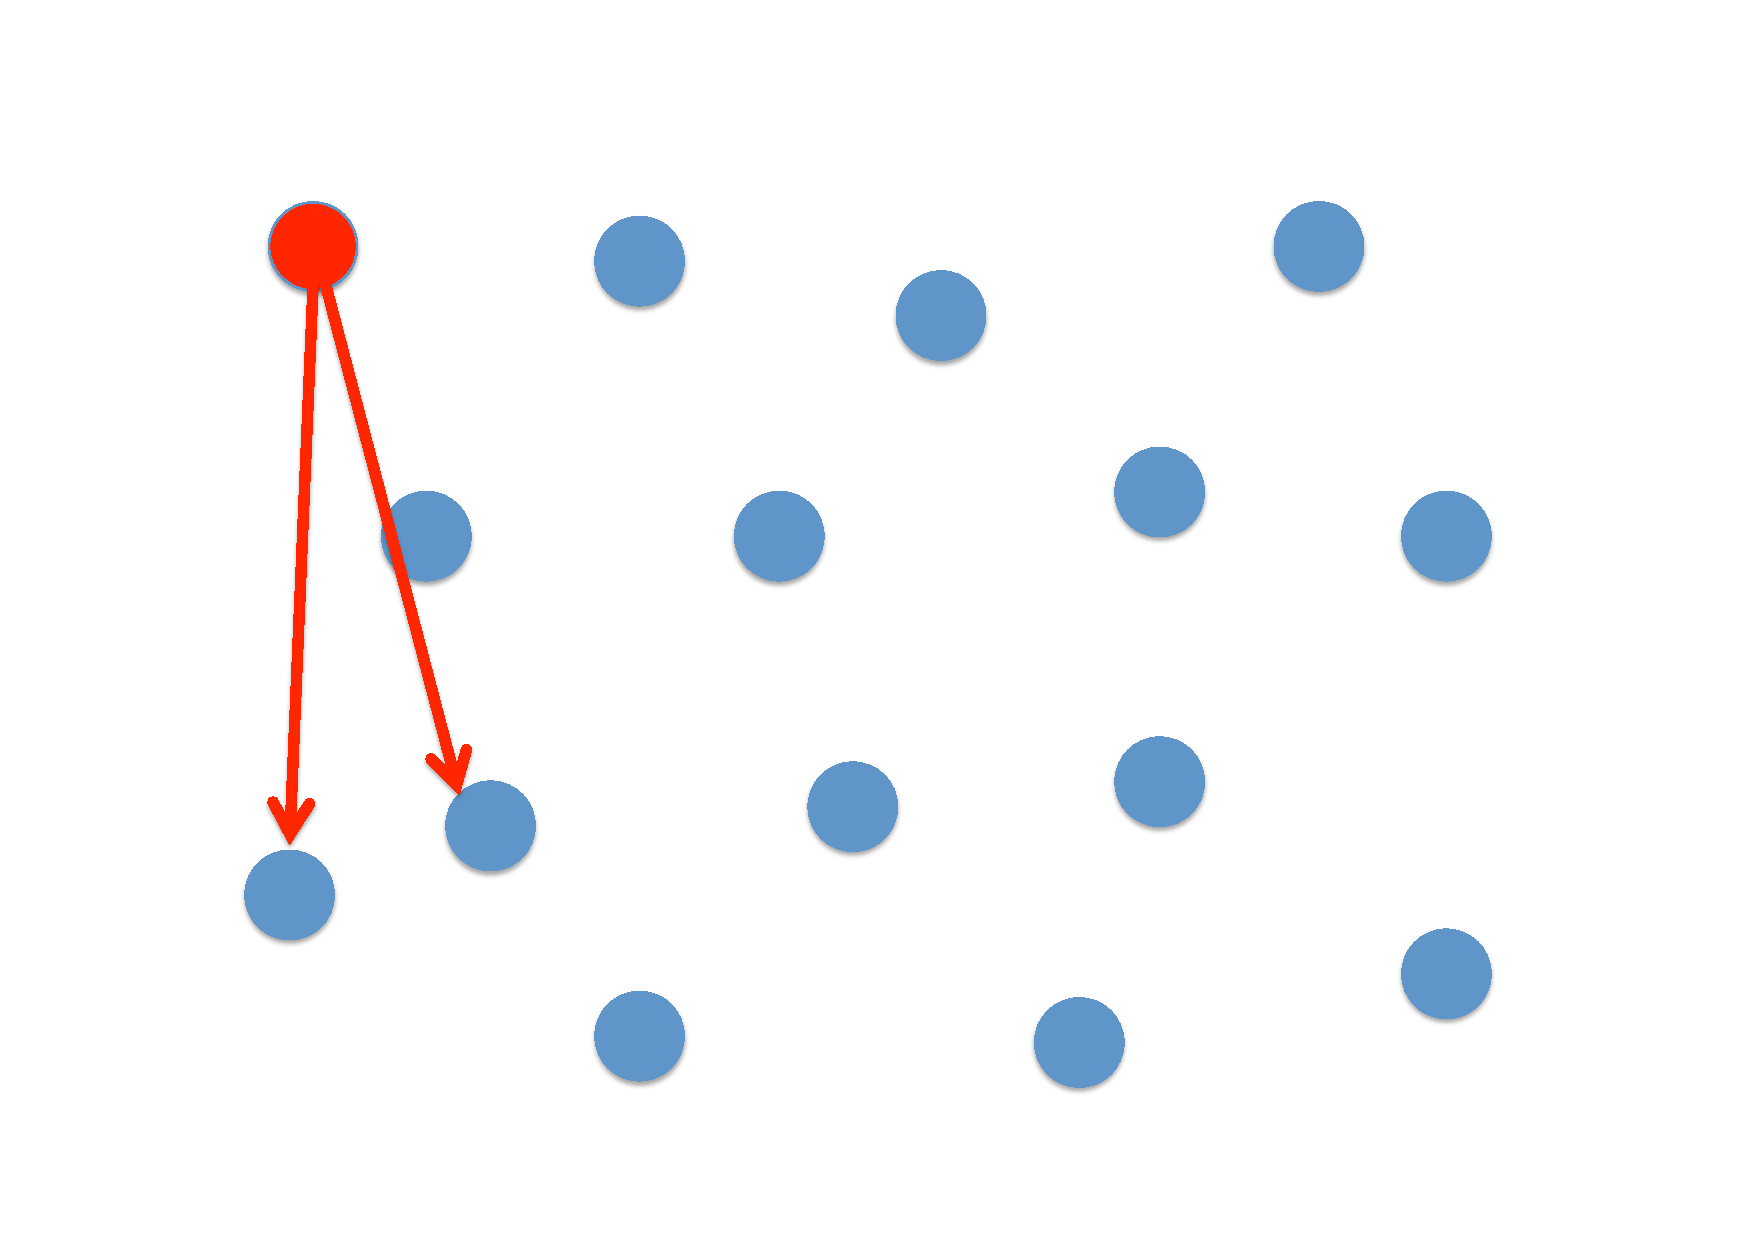
\includegraphics[width=1\textwidth]{pics/one2all4}
  \end{center}
\end{figure}

}

\frame{
\frametitle{The Academic View: Data Dissemination}
\framesubtitle{Design Alternatives: One to All}

\begin{figure}[h]
  \begin{center}
  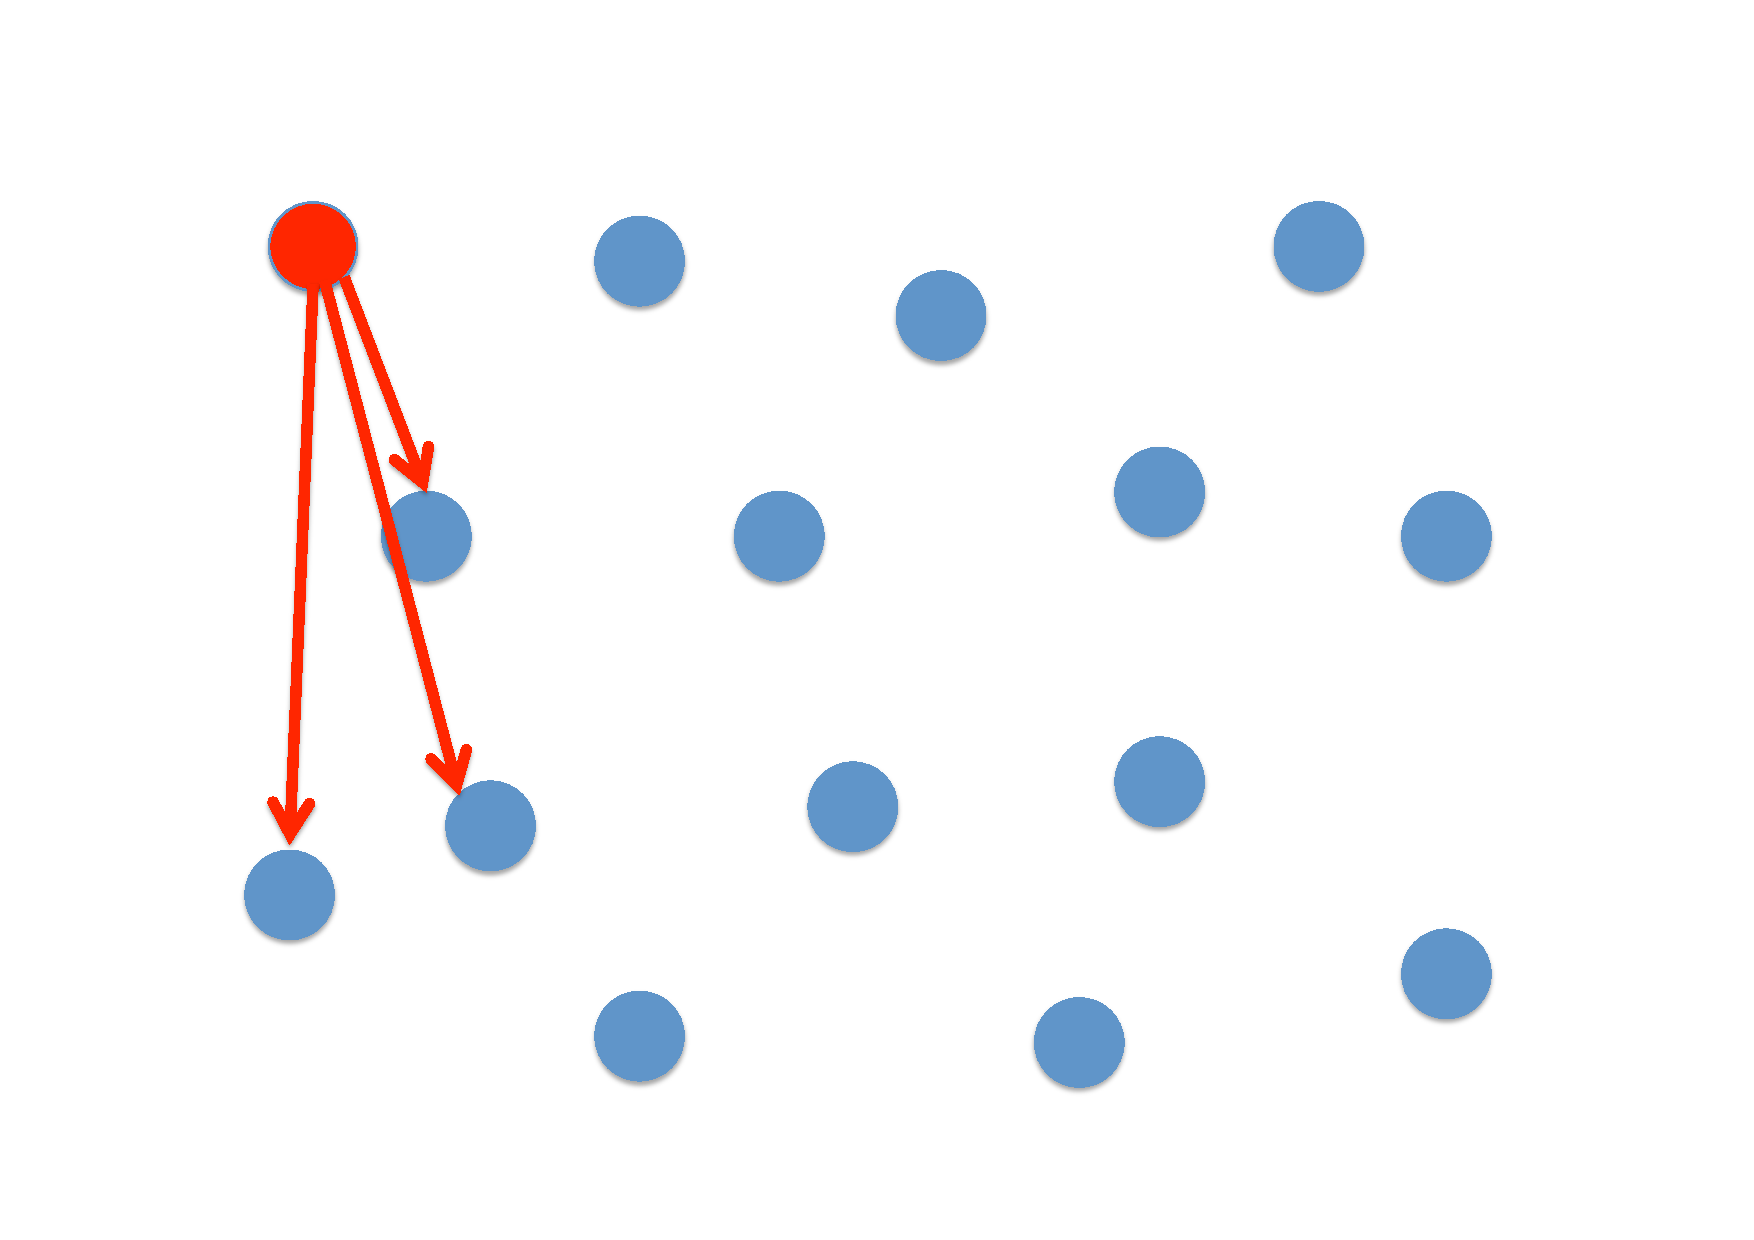
\includegraphics[width=1\textwidth]{pics/one2all5}
  \end{center}
\end{figure}

}

\frame{
\frametitle{The Academic View: Data Dissemination}
\framesubtitle{Design Alternatives: One to All}

\begin{figure}[h]
  \begin{center}
  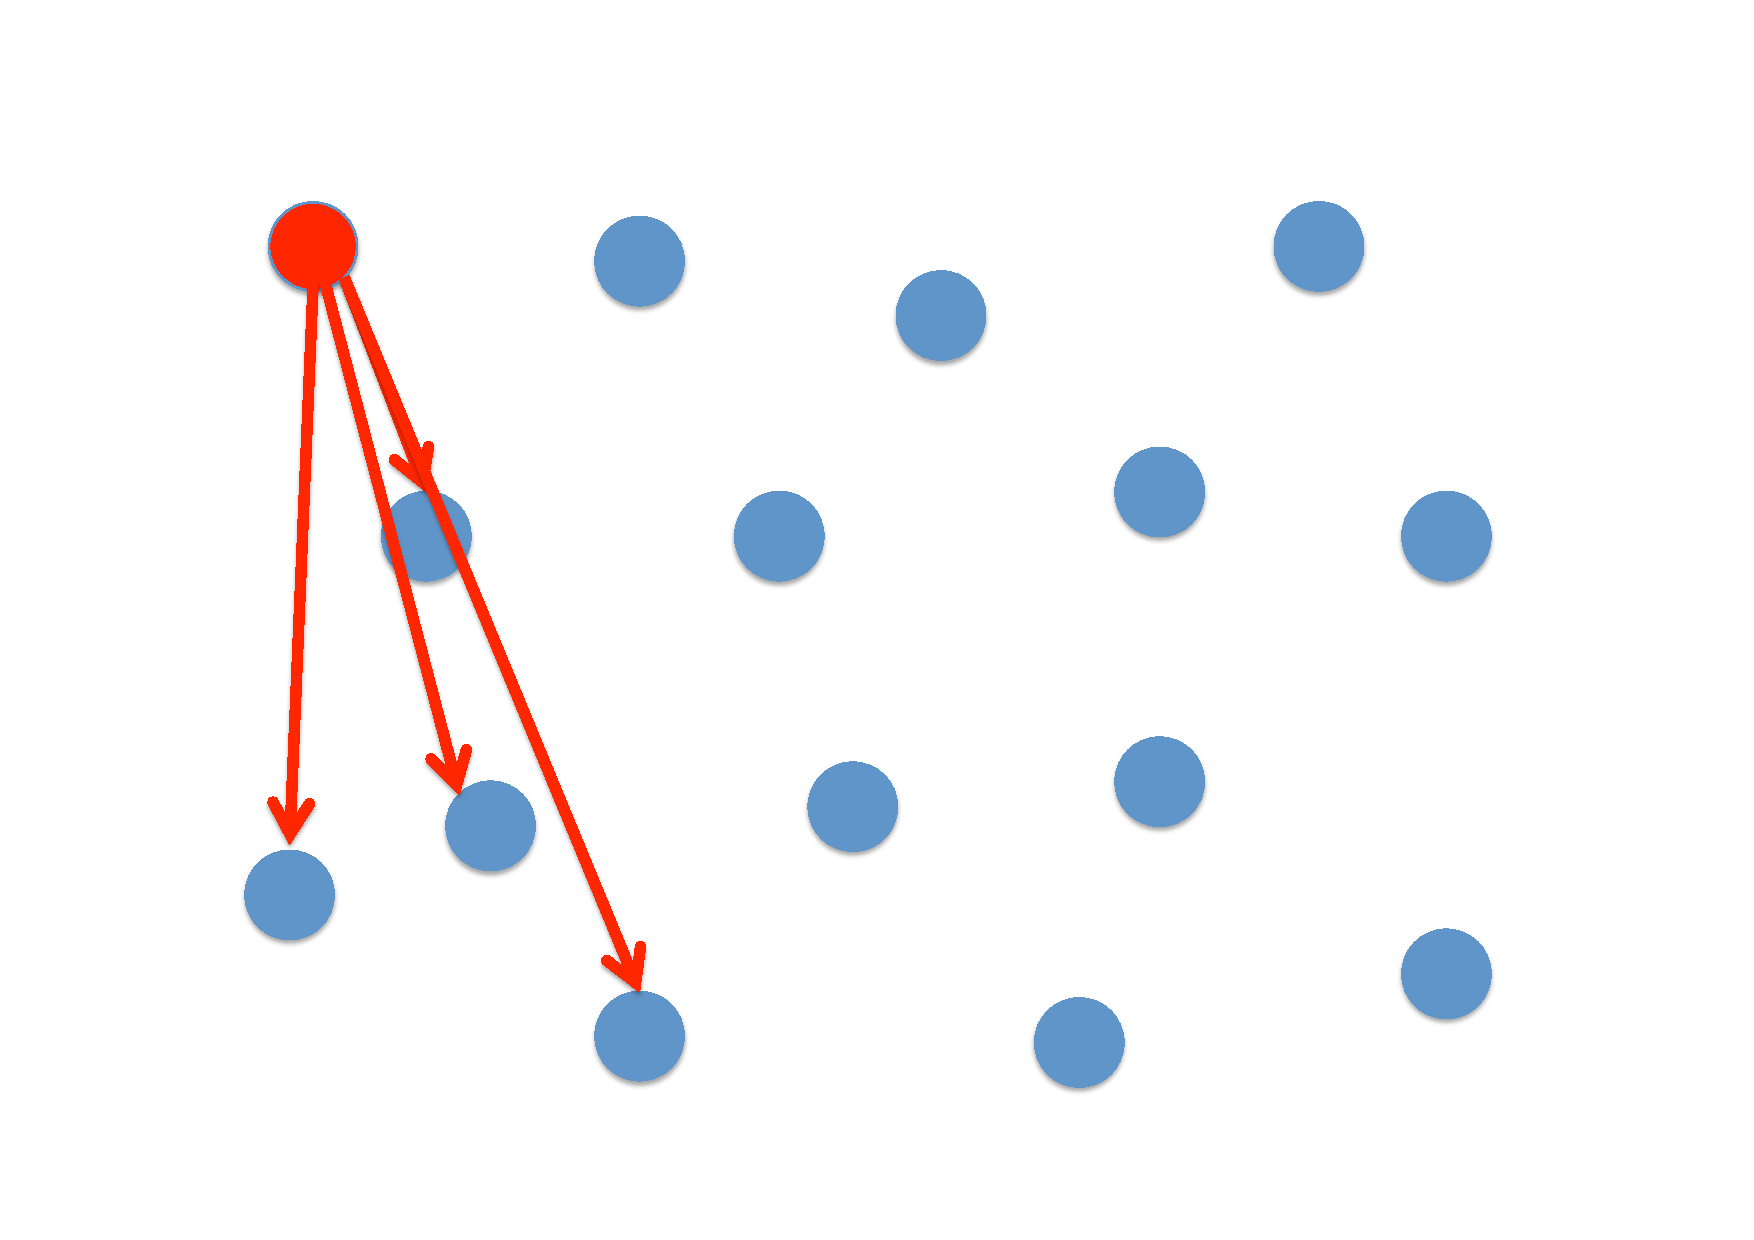
\includegraphics[width=1\textwidth]{pics/one2all6}
  \end{center}
\end{figure}

} 

\frame{
\frametitle{The Academic View: Data Dissemination}
\framesubtitle{Design Alternatives: One to All}

\begin{figure}[h]
  \begin{center}
  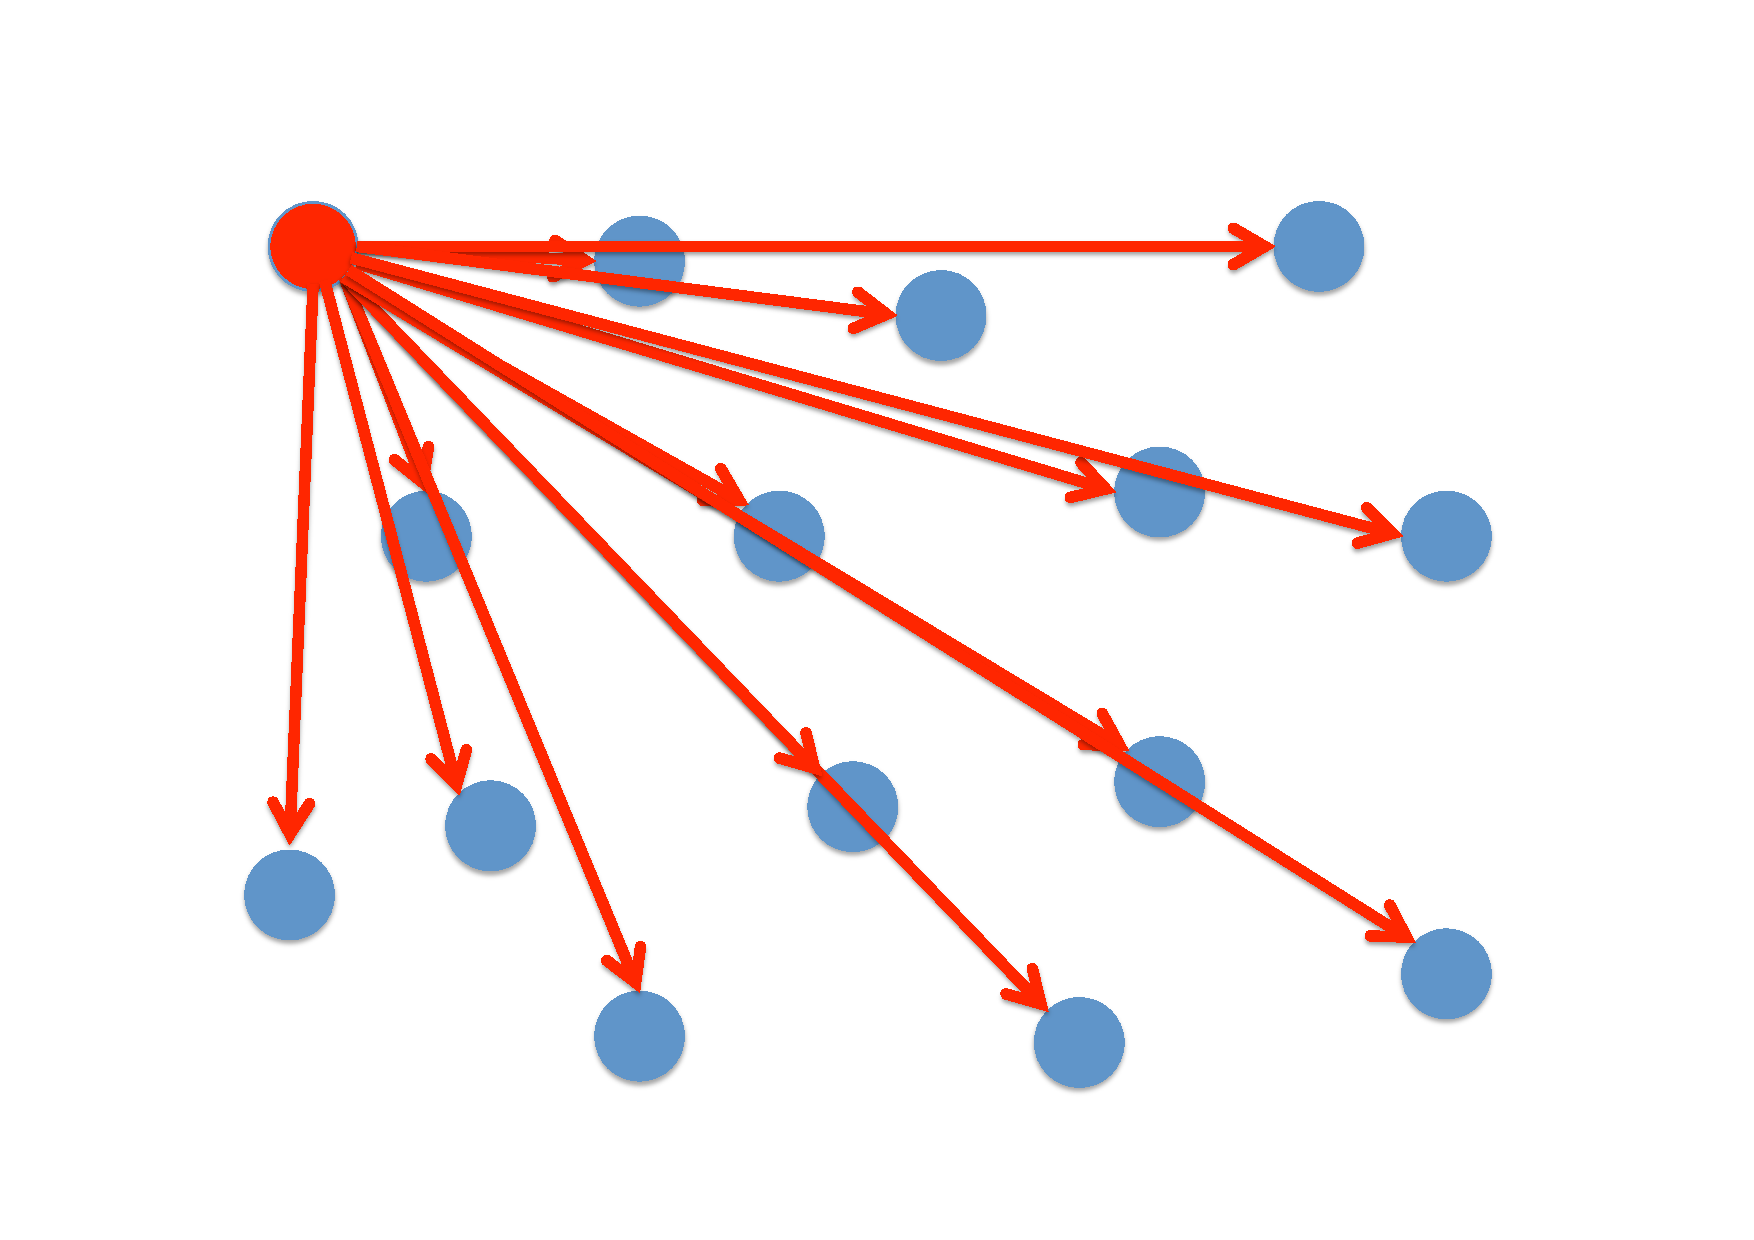
\includegraphics[width=1\textwidth]{pics/one2all7}
  \end{center}
\end{figure}

} 

\frame{
\frametitle{The Academic View: Data Dissemination}
\framesubtitle{Design Alternatives: One to All}

\begin{block}{One to All}
	\begin{itemize}
		\item Positive Aspects:
		\begin{itemize}
			\item Straight forward.
			\item No redundancy (i.e, each node receives each message a single time).
		\end{itemize}
	\end{itemize}
	
	\pause
	
	\begin{itemize}
		\item Negative Aspects:
		\begin{itemize}
			\item Requires each node to know the full membership.
			\item Not Scalable (no load distribution).
			\pause
			\item Not Resilient to Faults.
		\end{itemize}
	\end{itemize}
\end{block}
}

\frame{
\frametitle{The Academic View: Data Dissemination}
\framesubtitle{Design Alternatives: One to All}

\begin{figure}[h]
  \begin{center}
  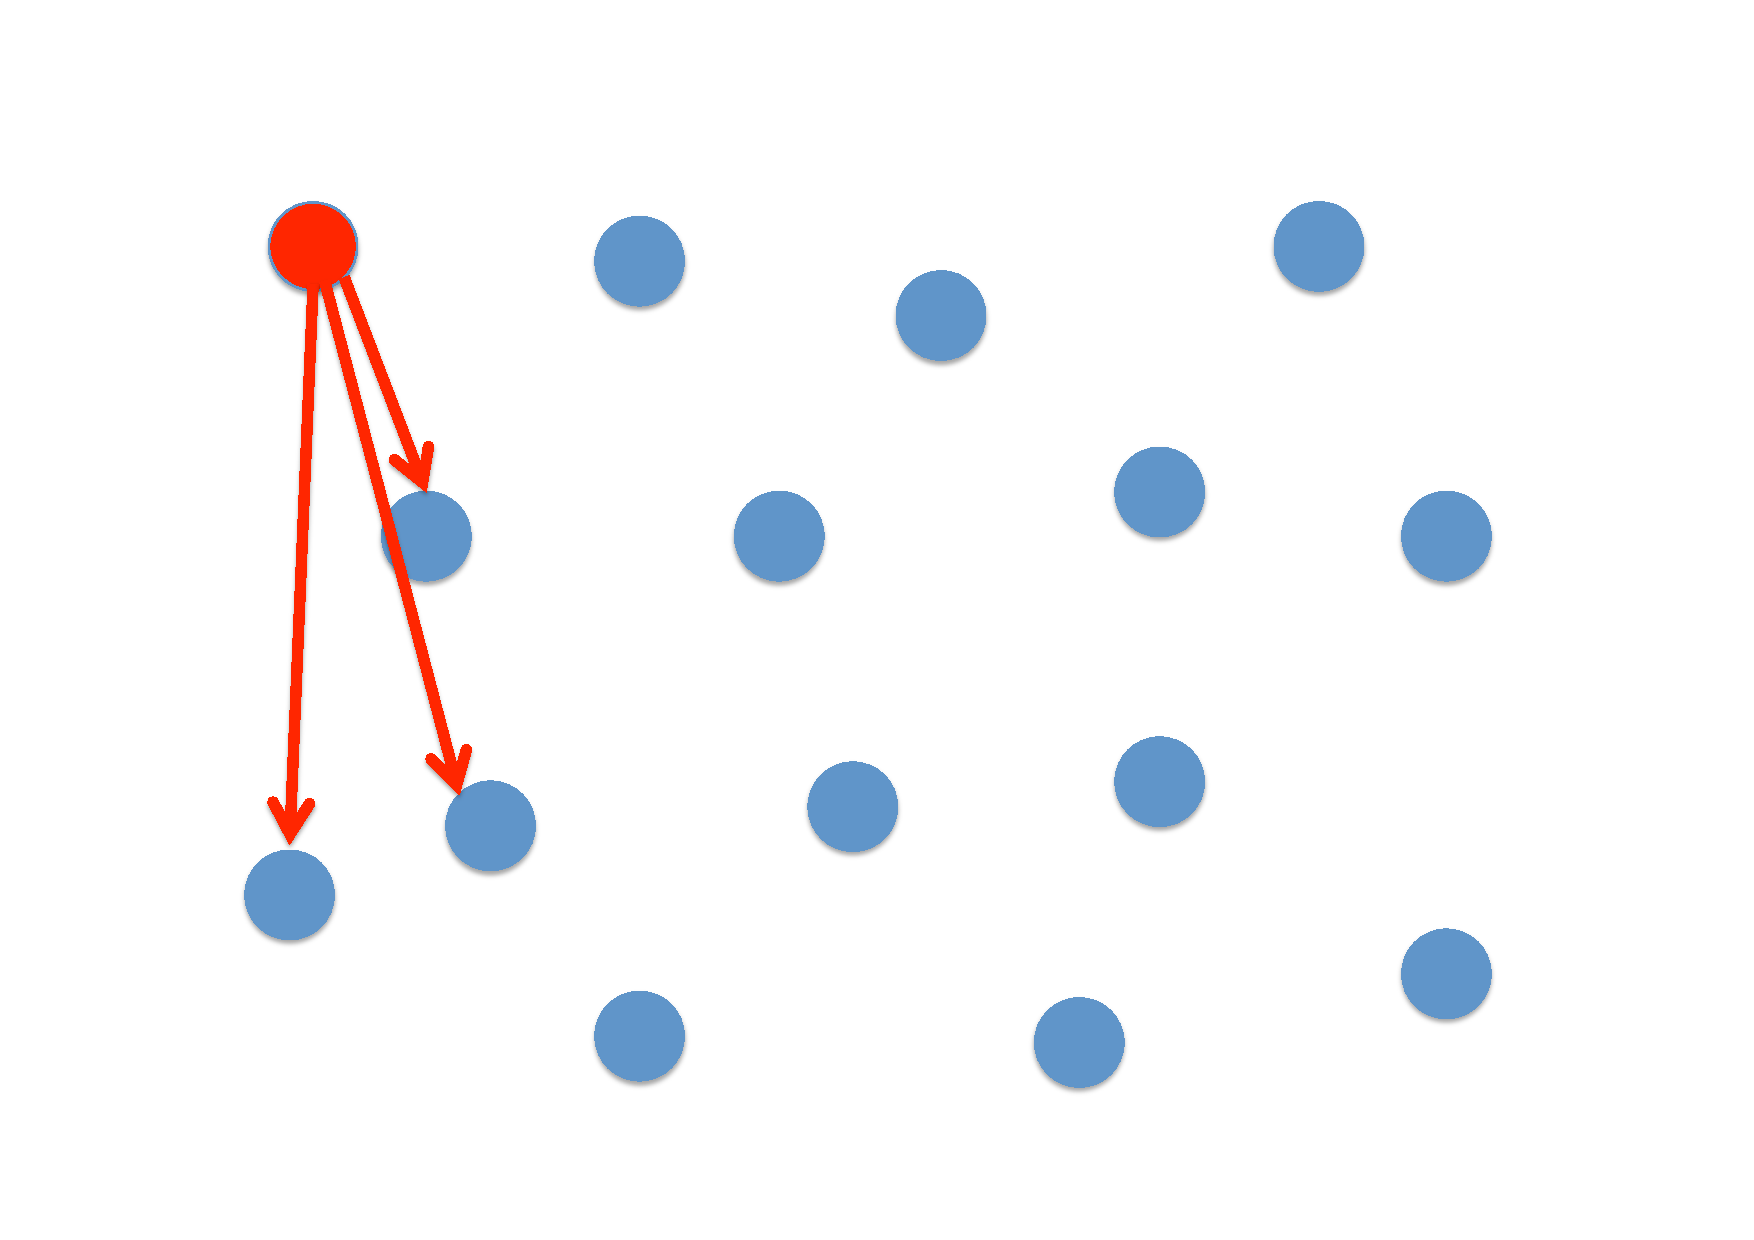
\includegraphics[width=1\textwidth]{pics/fault1}
  \end{center}
\end{figure}

}

\frame{
\frametitle{The Academic View: Data Dissemination}
\framesubtitle{Design Alternatives: One to All}

\begin{figure}[h]
  \begin{center}
  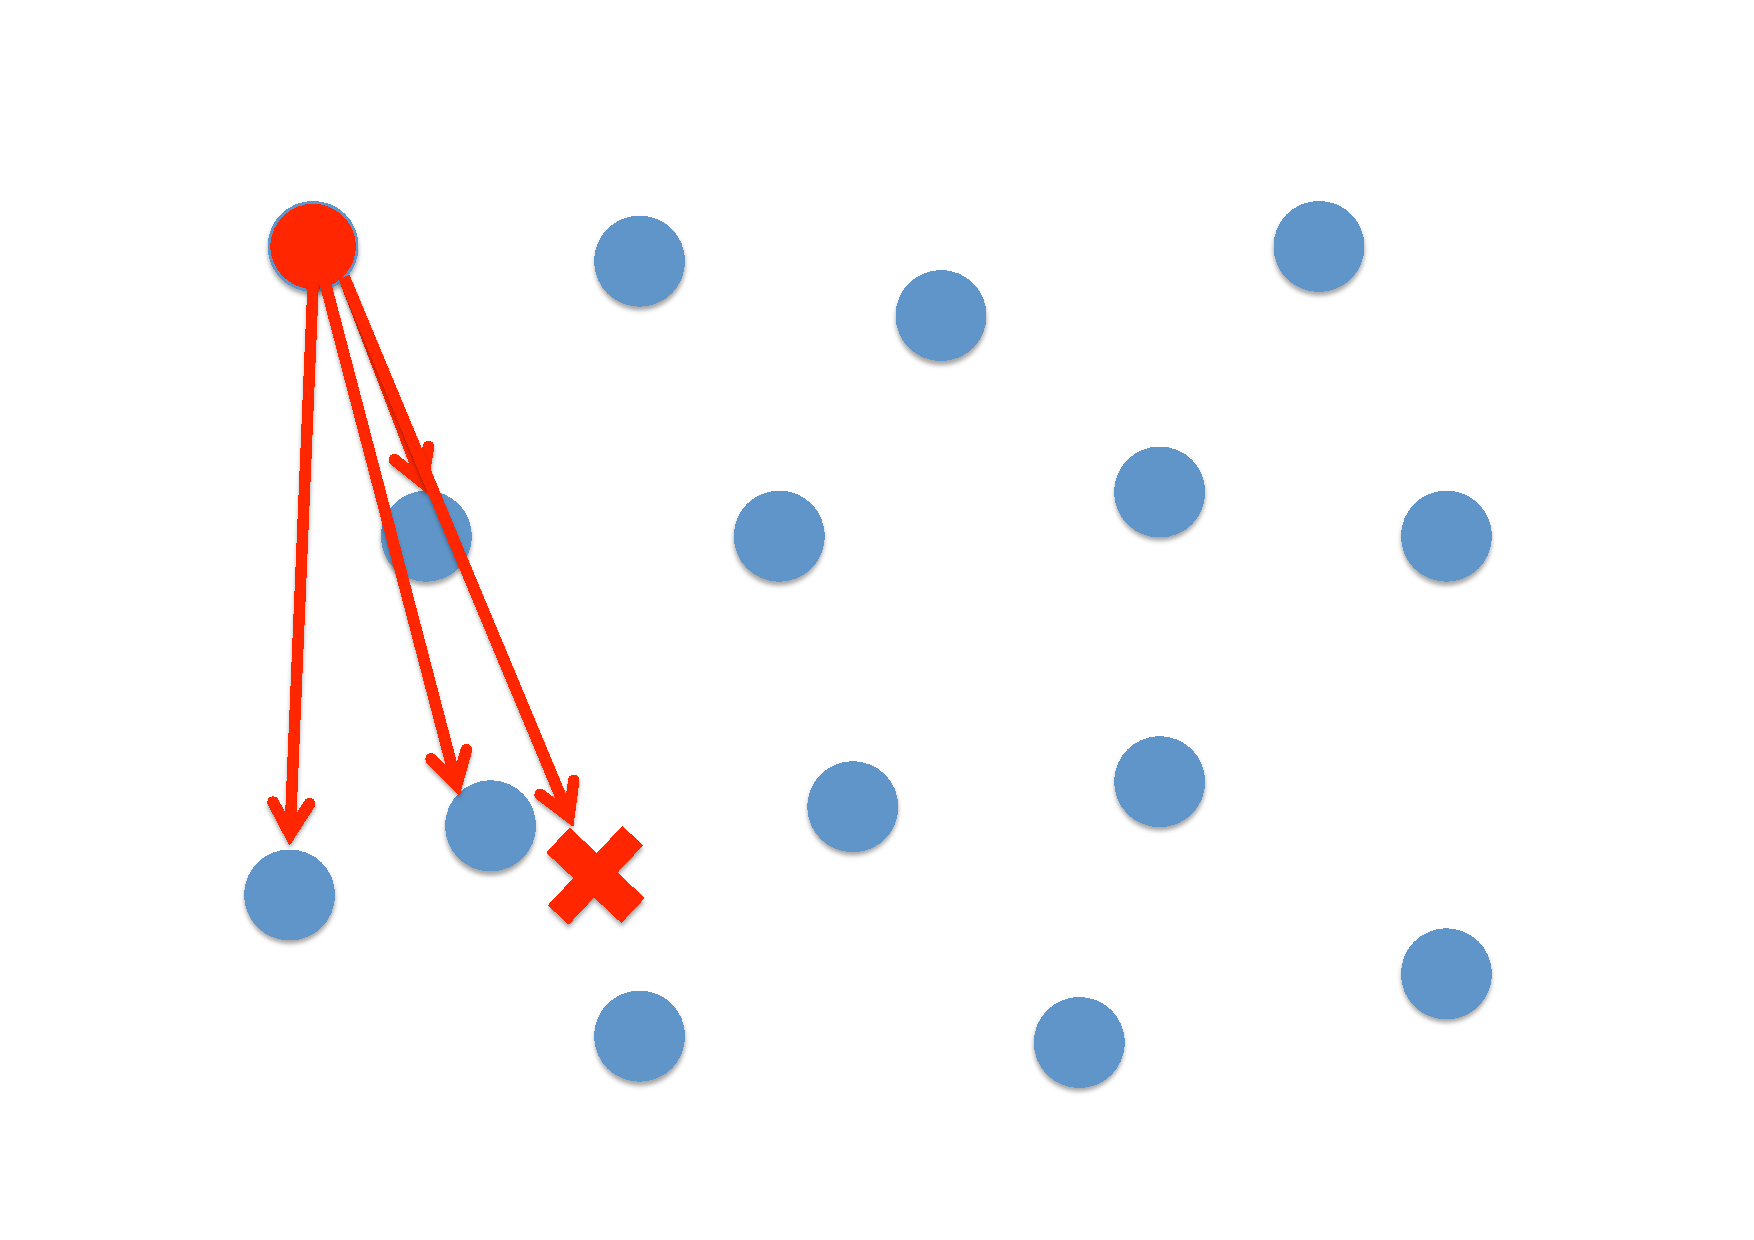
\includegraphics[width=1\textwidth]{pics/fault2}
  \end{center}
\end{figure}

}

\frame{
\frametitle{The Academic View: Data Dissemination}
\framesubtitle{Design Alternatives: One to All}

\begin{figure}[h]
  \begin{center}
  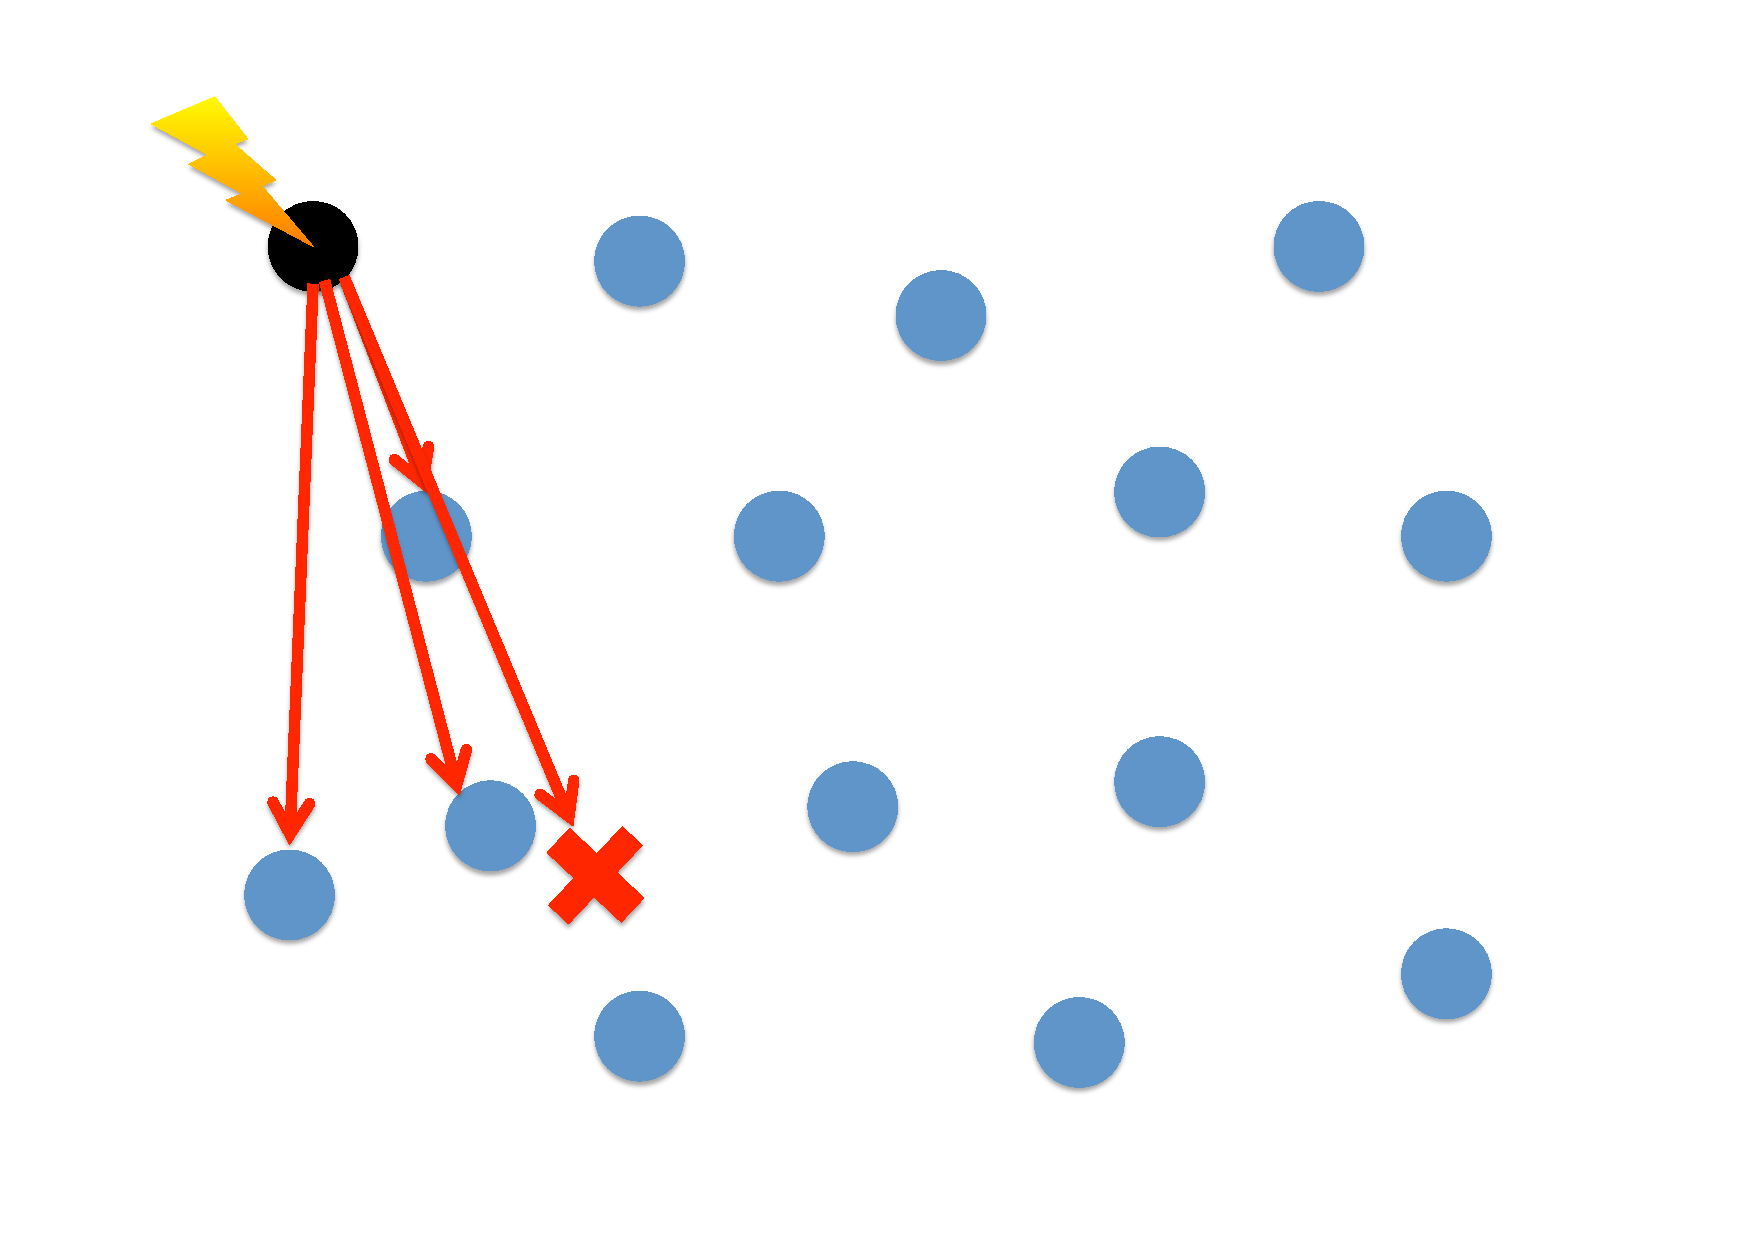
\includegraphics[width=1\textwidth]{pics/fault3}
  \end{center}
\end{figure}

}

\subsection{Design Alternatives: Spanning Tree}

\frame{
\frametitle{The Academic View: Data Dissemination}
\framesubtitle{Design Alternatives: Spanning Tree}

	\begin{block}{Dealing with Load Distribution}
		Organize participants/nodes in a tree and forward messages across the tree.
	\end{block}
	
	\pause
	
	~\\
	
	\begin{center}
	\huge{Spanning Treel}
	\end{center}

}

\frame{
\frametitle{The Academic View: Data Dissemination}
\framesubtitle{Design Alternatives: Spanning Tree}

\begin{figure}[h]
  \begin{center}
  \includegraphics[width=1\textwidth]{pics/spanningtree1}
  \end{center}
\end{figure}

}

\frame{
\frametitle{The Academic View: Data Dissemination}
\framesubtitle{Design Alternatives: Spanning Tree}

\begin{figure}[h]
  \begin{center}
  \includegraphics[width=1\textwidth]{pics/spanningtree2}
  \end{center}
\end{figure}

}

\frame{
\frametitle{The Academic View: Data Dissemination}
\framesubtitle{Design Alternatives: Spanning Tree}

\begin{figure}[h]
  \begin{center}
  \includegraphics[width=1\textwidth]{pics/spanningtree3}
  \end{center}
\end{figure}

}

\frame{
\frametitle{The Academic View: Data Dissemination}
\framesubtitle{Design Alternatives: Spanning Tree}

\begin{figure}[h]
  \begin{center}
  \includegraphics[width=1\textwidth]{pics/spanningtree4}
  \end{center}
\end{figure}

}

\frame{
\frametitle{The Academic View: Data Dissemination}
\framesubtitle{Design Alternatives: Spanning Tree}

\begin{figure}[h]
  \begin{center}
  \includegraphics[width=1\textwidth]{pics/spanningtree5}
  \end{center}
\end{figure}

}

\frame{
\frametitle{The Academic View: Data Dissemination}
\framesubtitle{Design Alternatives: Spanning Tree}

\begin{figure}[h]
  \begin{center}
  \includegraphics[width=1\textwidth]{pics/spanningtree6}
  \end{center}
\end{figure}

}

\frame{
\frametitle{The Academic View: Data Dissemination}
\framesubtitle{Design Alternatives: Spanning Tree}

\begin{figure}[h]
  \begin{center}
  \includegraphics[width=1\textwidth]{pics/spanningtree7}
  \end{center}
\end{figure}

}

\frame{
\frametitle{The Academic View: Data Dissemination}
\framesubtitle{Design Alternatives: Spanning Tree}

\begin{figure}[h]
  \begin{center}
  \includegraphics[width=1\textwidth]{pics/spanningtree8}
  \end{center}
\end{figure}

}

\frame{
\frametitle{The Academic View: Data Dissemination}
\framesubtitle{Design Alternatives: Spanning Tree}

\begin{figure}[h]
  \begin{center}
  \includegraphics[width=1\textwidth]{pics/spanningtree9}
  \end{center}
\end{figure}

}

\frame{
\frametitle{The Academic View: Data Dissemination}
\framesubtitle{Design Alternatives: Spanning Tree}

\begin{figure}[h]
  \begin{center}
  \includegraphics[width=1\textwidth]{pics/spanningtree10}
  \end{center}
\end{figure}

}

\frame{
\frametitle{The Academic View: Data Dissemination}
\framesubtitle{Design Alternatives: Spanning Tree}

\begin{figure}[h]
  \begin{center}
  \includegraphics[width=1\textwidth]{pics/spanningtree11}
  \end{center}
\end{figure}

}

\frame{
\frametitle{The Academic View: Data Dissemination}
\framesubtitle{Design Alternatives: Spanning Tree}

\begin{block}{Spanning Tree}
	\begin{itemize}
		\item Positive Aspects:
		\begin{itemize}
			\item Load Distribution.
			\item No redundancy (i.e, each node receives each message a single time).
		\end{itemize}
	\end{itemize}
	
	\pause
	
	\begin{itemize}
		\item Negative Aspects:
		\begin{itemize}
			\item Complexity in Managing the Topology (Hinders Scalability).
			\pause
			\item (Still) Not Resilient to Faults.
		\end{itemize}
	\end{itemize}
\end{block}
}

\frame{
\frametitle{The Academic View: Data Dissemination}
\framesubtitle{Design Alternatives: Spanning Tree}

\begin{figure}[h]
  \begin{center}
  \includegraphics[width=1\textwidth]{pics/spfault1}
  \end{center}
\end{figure}

}

\frame{
\frametitle{The Academic View: Data Dissemination}
\framesubtitle{Design Alternatives: Spanning Tree}

\begin{figure}[h]
  \begin{center}
  \includegraphics[width=1\textwidth]{pics/spfault2}
  \end{center}
\end{figure}

}

\frame{
\frametitle{The Academic View: Data Dissemination}
\framesubtitle{Design Alternatives: Spanning Tree}

\begin{figure}[h]
  \begin{center}
  \includegraphics[width=1\textwidth]{pics/spfault3}
  \end{center}
\end{figure}

}

\frame{
\frametitle{The Academic View: Data Dissemination}
\framesubtitle{Design Alternatives: Spanning Tree}

\begin{figure}[h]
  \begin{center}
  \includegraphics[width=1\textwidth]{pics/spfault4}
  \end{center}
\end{figure}

}

\frame{
\frametitle{The Academic View: Data Dissemination}
\framesubtitle{Design Alternatives: Spanning Tree}

\begin{figure}[h]
  \begin{center}
  \includegraphics[width=1\textwidth]{pics/spfault5}
  \end{center}
\end{figure}

}

\subsection{Design Alternatives: Flood}

\frame{
\frametitle{The Academic View: Data Dissemination}
\framesubtitle{Design Alternatives: Flood}

	\begin{block}{Dealing with Fault Tolerance}
		Organize participants/nodes in a random, highly connected, graph and forward messages across all links.
	\end{block}
	
	\pause
	
	~\\
	
	\begin{center}
	\huge{Flood}
	\end{center}

}

\frame{	
\frametitle{The Academic View: Data Dissemination}
\framesubtitle{Design Alternatives: Flood}
\begin{figure}[h]
  \begin{center}
  \includegraphics[width=1\textwidth]{pics/flood1}
  \end{center}
\end{figure}
}

\frame{	
\frametitle{The Academic View: Data Dissemination}
\framesubtitle{Design Alternatives: Flood}
\begin{figure}[h]
  \begin{center}
  \includegraphics[width=1\textwidth]{pics/flood2}
  \end{center}
\end{figure}
}

\frame{	
\frametitle{The Academic View: Data Dissemination}
\framesubtitle{Design Alternatives: Flood}
\begin{figure}[h]
  \begin{center}
  \includegraphics[width=1\textwidth]{pics/flood3}
  \end{center}
\end{figure}
}

\frame{	
\frametitle{The Academic View: Data Dissemination}
\framesubtitle{Design Alternatives: Flood}
\begin{figure}[h]
  \begin{center}
  \includegraphics[width=1\textwidth]{pics/flood4}
  \end{center}
\end{figure}
}

\frame{	
\frametitle{The Academic View: Data Dissemination}
\framesubtitle{Design Alternatives: Flood}
\begin{figure}[h]
  \begin{center}
  \includegraphics[width=1\textwidth]{pics/flood5}
  \end{center}
\end{figure}
}

\frame{	
\frametitle{The Academic View: Data Dissemination}
\framesubtitle{Design Alternatives: Flood}
\begin{figure}[h]
  \begin{center}
  \includegraphics[width=1\textwidth]{pics/flood6}
  \end{center}
\end{figure}
}

\frame{	
\frametitle{The Academic View: Data Dissemination}
\framesubtitle{Design Alternatives: Flood}
\begin{figure}[h]
  \begin{center}
  \includegraphics[width=1\textwidth]{pics/flood7}
  \end{center}
\end{figure}
}

\frame{	
\frametitle{The Academic View: Data Dissemination}
\framesubtitle{Design Alternatives: Flood}
\begin{figure}[h]
  \begin{center}
  \includegraphics[width=1\textwidth]{pics/flood8}
  \end{center}
\end{figure}
}

\frame{	
\frametitle{The Academic View: Data Dissemination}
\framesubtitle{Design Alternatives: Flood}
\begin{figure}[h]
  \begin{center}
  \includegraphics[width=1\textwidth]{pics/flood9}
  \end{center}
\end{figure}
}

\frame{	
\frametitle{The Academic View: Data Dissemination}
\framesubtitle{Design Alternatives: Flood}
\begin{figure}[h]
  \begin{center}
  \includegraphics[width=1\textwidth]{pics/flood10}
  \end{center}
\end{figure}
}


\frame{	
\frametitle{The Academic View: Data Dissemination}
\framesubtitle{Design Alternatives: Flood}
	\begin{block}{Flood}
	\begin{itemize}
		\item Positive Aspects:
		\begin{itemize}
			\item Load Distribution.
			\item Simple Design, and a random overlay is easier to maintain than a tree.
			\item Robust (due to inherent redudancy).
		\end{itemize}
	\end{itemize}
	
	\pause
	
	\begin{itemize}
		\item Negative Aspects:
		\begin{itemize}
			\item No longer that efficient (nodes receive and are required to process several copies of each message).
		\end{itemize}
	\end{itemize}
\end{block}
}

\frame{	
\frametitle{The Academic View: Data Dissemination}
\framesubtitle{Design Alternatives: Flood}
\begin{figure}[h]
  \begin{center}
  \includegraphics[width=1\textwidth]{pics/flood10}
  \end{center}
\end{figure}
}

\frame{	
\frametitle{The Academic View: Data Dissemination}
\framesubtitle{Design Alternatives: Flood}
\begin{figure}[h]
  \begin{center}
  \includegraphics[width=1\textwidth]{pics/flood11}
  \end{center}
\end{figure}
}

\subsection{Design Alternatives: Gossip}

\frame{
\frametitle{The Academic View: Data Dissemination}
\framesubtitle{Design Alternatives: Gossip}
	\begin{block}{Addressing Efficiency}
		Organize participants/nodes in a random, highly connected, graph and have nodes forward each message across a subset ($f$) of the links.
	\end{block}
	
	\pause
	
	~\\
	
	\begin{center}
	\huge{Gossip}
	\end{center}

}

\frame{
\frametitle{The Academic View: Data Dissemination}
\framesubtitle{Design Alternatives: Gossip}
\begin{figure}[h]
  \begin{center}
  \includegraphics[width=1\textwidth]{pics/gossip1}
  \end{center}
\end{figure}
}

\frame{
\frametitle{The Academic View: Data Dissemination}
\framesubtitle{Design Alternatives: Gossip}
\begin{figure}[h]
  \begin{center}
  \includegraphics[width=1\textwidth]{pics/gossip2}
  \end{center}
\end{figure}
}

\frame{
\frametitle{The Academic View: Data Dissemination}
\framesubtitle{Design Alternatives: Gossip}
\begin{figure}[h]
  \begin{center}
  \includegraphics[width=1\textwidth]{pics/gossip3}
  \end{center}
\end{figure}
}

\frame{
\frametitle{The Academic View: Data Dissemination}
\framesubtitle{Design Alternatives: Gossip}
\begin{figure}[h]
  \begin{center}
  \includegraphics[width=1\textwidth]{pics/gossip4}
  \end{center}
\end{figure}
}


\frame{
\frametitle{The Academic View: Data Dissemination}
\framesubtitle{Design Alternatives: Gossip}
\begin{figure}[h]
  \begin{center}
  \includegraphics[width=1\textwidth]{pics/gossip5}
  \end{center}
\end{figure}
}


\frame{
\frametitle{The Academic View: Data Dissemination}
\framesubtitle{Design Alternatives: Gossip}
\begin{figure}[h]
  \begin{center}
  \includegraphics[width=1\textwidth]{pics/gossip6}
  \end{center}
\end{figure}
}


\frame{
\frametitle{The Academic View: Data Dissemination}
\framesubtitle{Design Alternatives: Gossip}
\begin{figure}[h]
  \begin{center}
  \includegraphics[width=1\textwidth]{pics/gossip7}
  \end{center}
\end{figure}
}


\frame{
\frametitle{The Academic View: Data Dissemination}
\framesubtitle{Design Alternatives: Gossip}
\begin{figure}[h]
  \begin{center}
  \includegraphics[width=1\textwidth]{pics/gossip8}
  \end{center}
\end{figure}
}


\frame{
\frametitle{The Academic View: Data Dissemination}
\framesubtitle{Design Alternatives: Gossip}
\begin{figure}[h]
  \begin{center}
  \includegraphics[width=1\textwidth]{pics/gossip9}
  \end{center}
\end{figure}
}


\frame{
\frametitle{The Academic View: Data Dissemination}
\framesubtitle{Design Alternatives: Gossip}
\begin{figure}[h]
  \begin{center}
  \includegraphics[width=1\textwidth]{pics/gossip10}
  \end{center}
\end{figure}
}


\frame{
\frametitle{The Academic View: Data Dissemination}
\framesubtitle{Design Alternatives: Gossip}
\begin{figure}[h]
  \begin{center}
  \includegraphics[width=1\textwidth]{pics/gossip11}
  \end{center}
\end{figure}
}


\frame{
\frametitle{The Academic View: Data Dissemination}
\framesubtitle{Design Alternatives: Gossip}
\begin{figure}[h]
  \begin{center}
  \includegraphics[width=1\textwidth]{pics/gossip12}
  \end{center}
\end{figure}
}

\frame{
\frametitle{The Academic View: Data Dissemination}
\framesubtitle{Design Alternatives: Gossip}
	\begin{block}{Gossip}
	\begin{itemize}
		\item Positive Aspects:
		\begin{itemize}
			\item Load Distribution.
			\item Simple Design, and a random overlay is easier to maintain than a tree.
			\item Robust (due to inherent redudancy).
		\end{itemize}
	\end{itemize}
	
	\pause
	
	\begin{itemize}
		\item Negative Aspects:
		\begin{itemize}
			\item Slightly inefficient (but better than flood).
			\pause
			\item No longer predictable (each message will be disseminated across different links.
		\end{itemize}
	\end{itemize}
\end{block}
}

\subsection{Design Alternatives: Embedded Tree}

\frame{
\frametitle{The Academic View: Data Dissemination}
\framesubtitle{Design Alternatives: Embedded Tree}
	\begin{block}{All these design alternatives:}
		\begin{itemize}
			\item One-to-All.
			\item Spanning Tree.
			\item Flood.
			\item Gossip.
		\end{itemize}
	\end{block}
}

\frame{
\frametitle{The Academic View: Data Dissemination}
\framesubtitle{Design Alternatives: Embedded Tree}
	\begin{block}{All these design alternatives:}
		\begin{itemize}
			\item Spanning Tree.
			\item Flood.
			\item Gossip.
		\end{itemize}
	\end{block}
}

\frame{
\frametitle{The Academic View: Data Dissemination}
\framesubtitle{Design Alternatives: Embedded Tree}
	\begin{block}{All these design alternatives:}
		\begin{itemize}
			\item \textbf{Spanning Tree [Efficiency]}.
			\item Flood.
			\item Gossip.
		\end{itemize}
	\end{block}
}

\frame{
\frametitle{The Academic View: Data Dissemination}
\framesubtitle{Design Alternatives: Embedded Tree}
	\begin{block}{All these design alternatives:}
		\begin{itemize}
			\item \textbf{Spanning Tree [Efficiency]}.
			\item \textbf{Flood. [Robustness]}.
			\item \textbf{Gossip. [Robustness]}.
		\end{itemize}
	\end{block}
}

\frame{
\frametitle{The Academic View: Data Dissemination}
\framesubtitle{Design Alternatives: Embedded Tree}
	
	\center{
	\huge{
		At some point you start to see \textbf{trees} everywhere...
	}
	}
}

\frame{
\frametitle{The Academic View: Data Dissemination}
\framesubtitle{Design Alternatives: Embedded Tree}
	
\begin{figure}[h]
  \begin{center}
  \includegraphics[width=1\textwidth]{pics/floodtree1}
  \end{center}
\end{figure}
}

\frame{
\frametitle{The Academic View: Data Dissemination}
\framesubtitle{Design Alternatives: Embedded Tree}
	
\begin{figure}[h]
  \begin{center}
  \includegraphics[width=1\textwidth]{pics/floodtree2}
  \end{center}
\end{figure}
}

\frame{
\frametitle{The Academic View: Data Dissemination}
\framesubtitle{Design Alternatives: Embedded Tree}
	
\begin{figure}[h]
  \begin{center}
  \includegraphics[width=1\textwidth]{pics/floodtree3}
  \end{center}
\end{figure}
}

\frame{
\frametitle{The Academic View: Data Dissemination}
\framesubtitle{Design Alternatives: Embedded Tree}
	
\begin{figure}[h]
  \begin{center}
  \includegraphics[width=1\textwidth]{pics/floodtree4}
  \end{center}
\end{figure}
}

\frame{
\frametitle{The Academic View: Data Dissemination}
\framesubtitle{Design Alternatives: Embedded Tree}
	
\begin{figure}[h]
  \begin{center}
  \includegraphics[width=1\textwidth]{pics/floodtree5}
  \end{center}
\end{figure}
}

\frame{
\frametitle{The Academic View: Data Dissemination}
\framesubtitle{Design Alternatives: Embedded Tree}
	
\begin{figure}[h]
  \begin{center}
  \includegraphics[width=1\textwidth]{pics/gossiptree1}
  \end{center}
\end{figure}
}

\frame{
\frametitle{The Academic View: Data Dissemination}
\framesubtitle{Design Alternatives: Embedded Tree}
	
\begin{figure}[h]
  \begin{center}
  \includegraphics[width=1\textwidth]{pics/gossiptree2}
  \end{center}
\end{figure}
}

\frame{
\frametitle{The Academic View: Data Dissemination}
\framesubtitle{Design Alternatives: Embedded Tree}
	
\begin{figure}[h]
  \begin{center}
  \includegraphics[width=1\textwidth]{pics/gossiptree3}
  \end{center}
\end{figure}
}


\frame{
\frametitle{The Academic View: Data Dissemination}
\framesubtitle{Design Alternatives: Embedded Tree}
	
\begin{figure}[h]
  \begin{center}
  \includegraphics[width=1\textwidth]{pics/gossiptree4}
  \end{center}
\end{figure}
}


\frame{
\frametitle{The Academic View: Data Dissemination}
\framesubtitle{Design Alternatives: Embedded Tree}
	
\begin{figure}[h]
  \begin{center}
  \includegraphics[width=1\textwidth]{pics/gossiptree5}
  \end{center}
\end{figure}
}

\frame{
\frametitle{The Academic View: Data Dissemination}
\framesubtitle{Design Alternatives: Embedded Tree}

	\begin{block}{This observation:}
		Lead us to design the \textbf{Plumtree protocol}.
	\end{block}
%	
%	\pause
%	
%	\begin{figure}[h]
%  	\begin{center}
%	  \includegraphics[width=1\textwidth]{pics/plumtreecoauthors}
% 	 \end{center}
%	\end{figure}
}

\section{Embedded Tree: Plumtree Protocol}

\frame{
\frametitle{Embedded Trees: Plumtree Protocol}
\framesubtitle{Gossip modes of operation}
	
	\begin{block}{Eager push}
	Nodes send the message payload to random selected peers as soon as they receive a message for the first time.
%	\begin{itemize}
%		\item Lower latency.
%	\end{itemize}
\end{block}

\pause

\begin{block}{Lazy push}
	When a node receive a message for the first time, they only send that message identifier to random selected peers. If those peers have not received the message, they make an explicit request.
%	\begin{itemize}
%		\item Less redundant traffic.
%	\end{itemize}
\end{block}

\pause
\begin{itemize}
	\item Lazy push only makes sense with large payload sizes.
	\item There are trade-offs.
\end{itemize}
	
}

\frame{
\frametitle{Embedded Trees: Plumtree Protocol}

\framesubtitle{Overview}
	Plumtree: \textbf{p}ush-\textbf{l}azy-p\textbf{u}sh \textbf{m}ulticast \textbf{tree}.
	
	\begin{itemize}
	\item It operates as any gossip protocol, each node gossips with \emph{f} neighbors on top of a random overlay.
	\item Decentralized.
	\pause
	\item Creates (and maintain) an embedded tree on a random overlay.
	\item It combines two distinct gossip strategies:
	\begin{itemize}
		\item Eager Push: In the random overlay links that belong to the embedded spanning tree.
		\item Lazy Push: In the remaining random overlay links.
	\end{itemize}
	\pause
	\item TCP is used between nodes as it offers a better reliability and an additional fault detection mechanism.
	\end{itemize}

}

\frame{
\frametitle{Embedded Trees: Plumtree Protocol}
\framesubtitle{Building the Tree}

	\begin{itemize}
		\item Intuition: Use the links in the overlay that generated a message delivery.
		\pause
		\item After initialization all links in the overlay are candidates do belong to the spanning tree.
		\item When a message is broadcasted, all links used to disseminate a redundant message are pruned from the tree.
		\item If the random overlay is connected, after the dissemination of a message the tree will cover all nodes.
	\end{itemize}

}

\frame{
\frametitle{Embedded Trees: Plumtree Protocol}
\framesubtitle{Building the Tree}

	\begin{figure}[h]
  \begin{center}
  \includegraphics[width=0.9\textwidth]{exemplo/img1}
  \end{center}
	\end{figure}
}	

\frame{
\frametitle{Embedded Trees: Plumtree Protocol}
\framesubtitle{Building the Tree}

	\begin{figure}[h]
  \begin{center}
  \includegraphics[width=0.9\textwidth]{exemplo/img2}
  \end{center}
	\end{figure}
}	

\frame{
\frametitle{Embedded Trees: Plumtree Protocol}
\framesubtitle{Building the Tree}

	\begin{figure}[h]
  \begin{center}
  \includegraphics[width=0.9\textwidth]{exemplo/img3}
  \end{center}
	\end{figure}
}	

\frame{
\frametitle{Embedded Trees: Plumtree Protocol}
\framesubtitle{Building the Tree}

	\begin{figure}[h]
  \begin{center}
  \includegraphics[width=0.9\textwidth]{exemplo/img1}
  \end{center}
	\end{figure}
}	

\frame{
\frametitle{Embedded Trees: Plumtree Protocol}
\framesubtitle{Building the Tree}

	\begin{figure}[h]
  \begin{center}
  \includegraphics[width=0.9\textwidth]{exemplo/img4}
  \end{center}
	\end{figure}
}	

\frame{
\frametitle{Embedded Trees: Plumtree Protocol}
\framesubtitle{Building the Tree}

	\begin{figure}[h]
  \begin{center}
  \includegraphics[width=0.9\textwidth]{exemplo/img5}
  \end{center}
	\end{figure}
}	

\frame{
\frametitle{Embedded Trees: Plumtree Protocol}
\framesubtitle{Building the Tree}

	\begin{figure}[h]
  \begin{center}
  \includegraphics[width=0.9\textwidth]{exemplo/img6}
  \end{center}
	\end{figure}
}	

\frame{
\frametitle{Embedded Trees: Plumtree Protocol}
\framesubtitle{Building the Tree}

	\begin{figure}[h]
  \begin{center}
  \includegraphics[width=0.9\textwidth]{exemplo/img7}
  \end{center}
	\end{figure}
}	

\frame{
\frametitle{Embedded Trees: Plumtree Protocol}
\framesubtitle{Building the Tree}

	\begin{figure}[h]
  \begin{center}
  \includegraphics[width=0.9\textwidth]{exemplo/img8}
  \end{center}
	\end{figure}
}	

\frame{
\frametitle{Embedded Trees: Plumtree Protocol}
\framesubtitle{Building the Tree}

	\begin{figure}[h]
  \begin{center}
  \includegraphics[width=0.9\textwidth]{exemplo/img9}
  \end{center}
	\end{figure}
}	

\frame{
\frametitle{Embedded Trees: Plumtree Protocol}
\framesubtitle{Building the Tree}

	\begin{figure}[h]
  \begin{center}
  \includegraphics[width=0.9\textwidth]{exemplo/img10}
  \end{center}
	\end{figure}
}	

\frame{
\frametitle{Embedded Trees: Plumtree Protocol}
\framesubtitle{Recovering the Tree}

	\begin{itemize}
		\item If a node fails some nodes might become disconnected from the embedded tree.
		\item When a node receives a announcement for a payload message it did not received it starts a timer.
		\pause
		\item If the timer expires before receiving the payload message the node explicitly request the payload.
		\item Moves the node to whom it makes the request to its eagerPushPeers list.
		\pause
		\item The node that receives the request sends the payload.
		\item Moves the requester to its eagerPushPeers list.
		\pause
		\item At the end of this process the embedded tree is repaired.	
	\end{itemize}
}


\frame{
\frametitle{Embedded Trees: Plumtree Protocol}
\framesubtitle{Sharing the Tree}

	\begin{block}{Small number of senders}
		\begin{itemize}
			\item One Plumtree instance for each sender.
			\item Lower latency.
		\end{itemize}
	\end{block}

\pause

	\begin{block}{Large number of senders}
		\begin{itemize}
			\item One single Plumtree instance shared by all senders.
			\item Higher latency. 
		\end{itemize}
	\end{block}

}

\frame{
\frametitle{Embedded Trees: Plumtree Protocol}
\framesubtitle{Sharing the Tree}
	\begin{itemize}
		\item Initial motivation: Improve the latency with large number of senders.
		\pause
		\item Observations:
			\begin{itemize}
				\item New and better paths on the overlay might not be used for eager push.
				\item Tree repair process is random.
			\end{itemize}
		\pause
		\item Goal: Minimize the number of hops from sender to receiver.
	\end{itemize}
}

\frame{
\frametitle{Embedded Trees: Plumtree Protocol}
\framesubtitle{Sharing the Tree}
		\begin{figure}[h]
  \begin{center}
  \includegraphics[width=0.9\textwidth]{exemplo/img12}
  \end{center}
	\end{figure}
}

\frame{
\frametitle{Embedded Trees: Plumtree Protocol}
\framesubtitle{Sharing the Tree}
		\begin{figure}[h]
  \begin{center}
  \includegraphics[width=0.9\textwidth]{exemplo/img13}
  \end{center}
	\end{figure}
}

\frame{
\frametitle{Embedded Trees: Plumtree Protocol}
\framesubtitle{Sharing the Tree}
		\begin{figure}[h]
  \begin{center}
  \includegraphics[width=0.9\textwidth]{exemplo/img14}
  \end{center}
	\end{figure}
}

\frame{
\frametitle{Embedded Trees: Plumtree Protocol}
\framesubtitle{Sharing the Tree}
		\begin{figure}[h]
  \begin{center}
  \includegraphics[width=0.9\textwidth]{exemplo/img15}
  \end{center}
	\end{figure}
}

\frame{
\frametitle{Embedded Trees: Plumtree Protocol}
\framesubtitle{Experimental Evaluation}

\begin{itemize}
	\item Evaluation was conducted with the Peersim simulator.
	\item $10.000$ nodes system.
	\item Hundreds and hundreds of Simulations.
\end{itemize}

\pause

\begin{itemize}
	\item Compare the performance between:
	\begin{itemize}
		\item A standard (push) Gossip Protocol named \emph{Eager}
		\item Several configurations of Plumtree.
	\end{itemize}
\end{itemize}
}

\frame{
\frametitle{Embedded Trees: Plumtree Protocol}
\framesubtitle{Experimental Evaluation}
		
\begin{figure}[h]
  \begin{center}
  \includegraphics[width=1\textwidth]{pics/redundancy_stable}
  \end{center}
\end{figure}
}

\frame{
\frametitle{Embedded Trees: Plumtree Protocol}
\framesubtitle{Experimental Evaluation}
		\begin{figure}[h]
  \begin{center}
  \includegraphics[width=1\textwidth]{pics/max_hop_stable}
  \end{center}
	\end{figure}
}

\frame{
\frametitle{Embedded Trees: Plumtree Protocol}
\framesubtitle{Experimental Evaluation}
		\begin{figure}[h]
  \begin{center}
  \includegraphics[width=1\textwidth]{pics/reliability_agg}
  \end{center}
	\end{figure}
}

\section{The Industry View: Cluster Metadata Management}

\frame
{
	\frametitle{Outline}
{
\tiny
	\tableofcontents[currentsection,hideallsubsections]
}
}

\subsection{Global Information, Needed Locally}
\frame{
\frametitle{The Industry View: Cluster Metadata Management}
\framesubtitle{Global Information, Needed Locally}
\begin{block}{Operational Information}
  Mebership, Ownership, Transfers, Capabilities
\end{block}

\begin{block}{Configuration}
  Replica Counts, Backends, Is Feature X Enabled?
\end{block}

\begin{block}{Monitoring Data}
  Transfer Statistics, Background Work Tracking, Self-Monitoring
\end{block}
}

\subsection{Requirements}
\frame{
\frametitle{The Industry View: Cluster Metadata Management}
\framesubtitle{Requirements}
\begin{itemize}
  \item Failure Tolerance
  \begin{itemize}
    \item Disable malicious clients despite network partitions
    \item Add new nodes despite others being down
  \end{itemize}
  \pause
  \item Quick Convergence
  \begin{itemize}
    \item Become aware of new nodes ASAP
    \item Keep monitoring data as fresh as possible
  \end{itemize}
  \pause
  \item Minimal Resource Usage
  \begin{itemize}
    \item Goal is to speed up, not slow down, foreground work
    \item Network is needed for the data!
  \end{itemize}
  \pause
  \item AP typically, CP rarely necessary
\end{itemize}
}

%To Jordan: Add your sub sections / main slides here
\section{Cluster Metadata Management In Riak}

\frame
{
	\frametitle{Outline}
{
\tiny
	\tableofcontents[currentsection,hideallsubsections]
}
}

%To Jordan: Add your sub sections / main slides here

\subsection{Implementations}
\frame{
\frametitle{Cluster Metadata Management In Riak}
\framesubtitle{Implementations}
\begin{block}{0.x}
\begin{itemize}
  \item Peer Service: Classic Anti-Entropy Protocol
  \item Data Dissemination: Same
\end{itemize}
\end{block}
\begin{block}{1.x}
\begin{itemize}
  \item Peer Service: Static Graph Overlay w/ Anti-Entropy
  \item Data Dissemination: Same
\end{itemize}
\end{block}
\begin{block}{2.x}
\begin{itemize}
  \item Peer Service: Static Graph Overlay w/ Anti-Entropy
  \item Data Dissemination: Sender-Based Embedded Trees
\end{itemize}
\end{block}
}

\subsection{Motivations}
\frame{
\frametitle{Cluster Metadata Management In Riak}
\framesubtitle{Motivations}
\begin{block}{0.x to 1.0}
\begin{itemize}
  \item Anti-Entropy is Reliable but Slow to Converge
  \item Improve Convergence Time, Specifically in Failure Scenarios
\end{itemize}
\end{block}
\begin{block}{1.x to 2.0}
\begin{itemize}
  \item Static Graph Overlay/Anti-Entropy have several issues:
    \begin{itemize}
      \item Too Much Network Overhead
      \item Improved Convergence Only Needed for Subset of Data
      \item Cold Rumor Mongering
    \end{itemize}
  \item Improve Resource Usage and Stability
\end{itemize}
\end{block}
}

\subsection{Plumtree: From Academia to Industry}
\frame{
\frametitle{Cluster Metadata Management In Riak}
\framesubtitle{Plumtree: From Academia to Industry}
\begin{block}{Connectivity}
``all nodes should have in their partial views...another correct node'' is not an invariant we can maintain
\end{block}
\begin{block}{System Model}
Must consider dropped, delayed, duplicated* messages in addition to node failures
\end{block}
\begin{block}{Topology}
Peer Service is Fully Connected (as is Erlang)
\end{block}
\begin{block}{Membership}
Operator-controlled instead of reactive (failure detector is implemented separately from peer service)
\end{block}
}

\subsection{Extending Plumtree}
\frame{
\frametitle{Cluster Metadata Management In Riak}
\framesubtitle{Extending Plumtree}
\begin{block}{What happens if Lazy Messages are Dropped?}
Add to Outstanding Set. Remove on Graft or Ack
\end{block}
\begin{block}{Handling Extreme Failures}
Back protocol by random anti-entropy with peers that are not in eager or lazy sets
\end{block}
\begin{block}{Shared vs. Sender-Based Trees}
Sender-Based. Minimize overhead w/ Lazy Construction
\end{block}
}

\subsection{Measurements}
\frame{
\frametitle{Cluster Metadata Management In Riak}
\framesubtitle{Measurements}
\begin{itemize}
\item Reduced convergence time (measured in LDH) by 66\%
\item Reduced needless message overhead in stable state 99.9\%
\item \% Failures before needing to rely on anti-entropy good for small clusters (near 90\%) but decreased quickly for larger clusters (under 50\%)
\end{itemize}
}

\subsection{Peer Service Tuning}
\frame{
\frametitle{Cluster Metadata Management In Riak}
\framesubtitle{Peer Service Tuning}
\begin{itemize}
\item Want to increase percent failures we can tolerate before relying on anti-entropy
\item Fanout of tree given to us by peer service matters
\item For clusters > 10 nodes, fanout = ln(cluster size) + 1
\item With our use of multiple trees, more peer service tuning may be necessary
\end{itemize}
}


\section{The Academic View: When One Tree is not Enough}

\frame
{
	\frametitle{Outline}
{
\tiny
	\tableofcontents[currentsection,hideallsubsections]
}
}

\subsection{Understanding The Problem}

\frame{
\frametitle{The Academic View: When One Tree is not Enough}
\framesubtitle{Understanding The Problem}

	\begin{block}{We had Plumtree:}
		\begin{itemize}
		\item Efficient.
		\item Very Robust.
		\item Could even rebalance itself to improve latency (height of the tree).
		\end{itemize}
	\end{block}

	\pause

	\begin{block}{The reality about trees...}
		Trees do not distribute the load evenly among participants.
	\end{block}

}

\frame{
\frametitle{The Academic View: When One Tree is not Enough}
\framesubtitle{Understanding The Problem}
	
\begin{figure}[h]
  \begin{center}
  \includegraphics[width=1\textwidth]{pics/nobalance1}
  \end{center}
\end{figure}
}

\frame{
\frametitle{The Academic View: When One Tree is not Enough}
\framesubtitle{Understanding The Problem}
	
\begin{figure}[h]
  \begin{center}
  \includegraphics[width=1\textwidth]{pics/nobalance2}
  \end{center}
\end{figure}
}

\frame{
\frametitle{The Academic View: When One Tree is not Enough}
\framesubtitle{Understanding The Problem}
	
\begin{figure}[h]
  \begin{center}
  \includegraphics[width=1\textwidth]{pics/nobalance3}
  \end{center}
\end{figure}
}

\frame{
\frametitle{The Academic View: When One Tree is not Enough}
\framesubtitle{Understanding The Problem}
	
\begin{figure}[h]
  \begin{center}
  \includegraphics[width=1\textwidth]{pics/nobalance4}
  \end{center}
\end{figure}
}

\subsection{Naive Solutions}

\frame{
\frametitle{The Academic View: When One Tree is not Enough}
\framesubtitle{Naive Solutions}

	\begin{block}{How hard can this be?}
		\begin{itemize}
			\item We started by experimenting with two simple approaches:
			\item NUTS: Naive Unstructured spliTStream
			\item BOLTS: Basic multiple Overlay-TreeS
		\end{itemize}
	\end{block}
}

\frame{
\frametitle{The Academic View: When One Tree is not Enough}
\framesubtitle{Naive Solutions: NUTS}

      \begin{itemize}
        \item Pick  $t$ nodes at random and create  $t$  Plumtrees; each
          rooted at a different node.
      \end{itemize}
      \begin{center}
	\pgfimage<1>[width=7cm]{figs/nuts/nuts1}
         \pgfimage<2>[width=7cm]{figs/nuts/nuts2}
         \pgfimage<3>[width=7cm]{figs/nuts/nuts3}
      \end{center}
}

\frame{
\frametitle{The Academic View: When One Tree is not Enough}
\framesubtitle{Naive Solutions: BOLTS}

  \begin{itemize}
    \item Create $t$ different unstructured overlays and create a
      Plumtree using each overlay.
  \end{itemize}
  
  \pgfimage<1>[width=5.5cm]{figs/bolts/bolts1}
  \pgfimage<1>[width=5.5cm]{figs/bolts/bolts2}
  \pgfimage<2>[width=5.5cm]{figs/bolts/bolts3}
  \pgfimage<2>[width=5.5cm]{figs/bolts/bolts4}

}

\frame{
\frametitle{The Academic View: When One Tree is not Enough}
\framesubtitle{Naive Solutions: NUTS \& BOLTS}

  \begin{center}
  \pgfimage[width=10cm]{figs/motivation/interior}
  \end{center}

}

\subsection{Understanding The Goal}

\frame{
\frametitle{The Academic View: When One Tree is not Enough}
\framesubtitle{Understanding The Goal}
  
  \begin{block}{From one tree to multiple trees}
  
  \begin{itemize}
    \item Load balancing:
    \begin{itemize}
    \item every node should be interior on the same number of trees
    \end{itemize}
    \item Use all resources:
    \begin{itemize}
      \item each node should be interior in at least one tree
    \end{itemize}
    \item Fault-tolerance:
    \begin{itemize}
      \item each node should be interior in at most one tree
    \end{itemize}
  \end{itemize}
  
  \end{block}
}



\section{The Thicket Protocol}

\frame
{
	\frametitle{Outline}
{
\tiny
	\tableofcontents[currentsection,hideallsubsections]
}
}

\subsection{Deploying the Trees}

\frame{
\frametitle{The Thicket Protocol}
\framesubtitle{Deploying the Trees}

	\begin{itemize}
		\item We use the same principle as in Plumtree to define trees, however:
		\begin{itemize}
			\item Overlay links are explicitly added to each tree (instead of removed).
			\item Trees are deployed by taking into consideration the remaining trees.
			\pause
			\item Finding the minimal coordination necessary to achieve our goal is tricky.
			\pause
			\item Tree coverage is impossible at tree deployment time.
		\end{itemize}
	\end{itemize}

}

\subsection{Recovering Trees}

\frame{
\frametitle{The Thicket Protocol}
\framesubtitle{Recovering Trees}

	\begin{itemize}
		\item Global coverage of trees is ensured by the repair mechanism.
		\pause
		\item All messages exchanged among nodes convey information about the load of the sender.
		\begin{itemize}
			\item How many messages it sends per time unit.
			\item How many child nodes in each tree.
		\end{itemize}
		\item Tree repair uses less loaded nodes.
	\end{itemize}

}

\subsection{Experimental Results}

\frame{
\frametitle{The Thicket Protocol}
\framesubtitle{Experimental Results}
\begin{itemize}
    \item Simulated a 10.000 overlay using PeerSim.
    \item Comparison with NUTS and  BOLTS (and Plumtree).
    \item Same underlying unstructured overlay network.
    \item Assumes reliable FIFO channels.
  \end{itemize}
}

\frame{
\frametitle{The Thicket Protocol}
\framesubtitle{Experimental Results}

 \begin{center}
  \pgfimage[width=10cm]{figs/interior}
  \end{center}
}

\frame{
\frametitle{The Thicket Protocol}
\framesubtitle{Experimental Results}

  \begin{center}
  \pgfimage<2>[width=9cm]{figs/reliabilityr}
  \end{center}

}

\section{The Industry View: Improving Cluster Metadata Management}

%To Jordan: Add your sub sections / main slides here

\frame
{
	\frametitle{Outline}
{
\tiny
	\tableofcontents[currentsection,hideallsubsections]
}
}

\subsection{Measuring Interior Nodes}
\frame{
\frametitle{The Industry View: Improving Cluster Metadata Management}
\framesubtitle{Measuring Interior Nodes}
\begin{block}{10 Nodes}
  \begin{itemize}
    \item 4 of 10 nodes are interior in 3 of 10 trees
    \item 3 of 10 nodes are interior in 4 of 10 trees
    \item 3 of 10 nodes are interior in 5 of 10 trees
  \end{itemize}
\end{block}
\begin{block}{20 Nodes}
  \begin{itemize}
    \item 4 nodes are interior only when roots
    \item 16 nodes are interior in 5 or more trees
  \end{itemize}
\end{block}
\begin{block}{80 Nodes}
  \begin{itemize}
    \item 4 nodes are interior only when roots
    \item 36 of 80 nodes are interior in > 25\% of trees
  \end{itemize}
\end{block}
}

\subsection{The Peer Service's Role}
\frame{
\frametitle{The Industry View: Improving Cluster Metadata Management}
\framesubtitle{Improving Interior Node Counts}
\begin{itemize}
\item Coupling between fanout, number of trees, and how many times a node must be interior
\item Height of initial trees constructed by peer service
\end{itemize}
}


\section{The Future of Cluster Metadata in Riak}

%To Jordan: Add your sub sections / main slides here

\frame
{
	\frametitle{Outline}
{
\tiny
	\tableofcontents[currentsection,hideallsubsections]
}
}


\subsection{Expand Usage}
\frame{
\frametitle{The Future of Cluster Metadata in Riak}
\framesubtitle{Expand Usage}
\begin{block}{Exploring Thicket}
\begin{itemize}
  \item Research Area
\end{itemize}
\end{block}
\begin{block}{Migration \& New Data}
\begin{itemize}
  \item Move data from 1.x subsystem to 2.x subsystem
  \item Store data we couldn't before
\end{itemize}
\end{block}
\begin{block}{WAN Replication}
\begin{itemize}
  \item Integrate with Riak's Multi-Site Replication
  \item Abstract Messaging Layer
\end{itemize}
\end{block}
}

\section{Summary}

\frame
{
	\frametitle{Outline}
{
\tiny
	\tableofcontents[currentsection,hideallsubsections]
}
}

\frame{
\frametitle{Summary}
\framesubtitle{}

}

\frame
{
	\frametitle{}
	\framesubtitle{}

	\begin{center}
		{\Huge
			Thanks.
		}
	\end{center}
}

\end{document}
